% AUTHOR: Ruslan Kiianchuk <ruslan.kiianchuk@gmail.com>


\chapter{Algebraic analysis of symmetric block ciphers}
\label{sec:algebraic}

Being a fairly new technique, algebraic cryptanalysis is one of the most
promissory and powerful methods for analysing cryptographic
algorithms~\cite{Albrecht2010}. It implies modeling a cryptographic algorithm
by a set of algebraic equations that form multivariate polynomial equations
system over finite field. The lower degree such system has the easier it is to
solve, so it is a rule of thumb in algebraic analysis to construct algebraic
systems that contain only quadratic multivariate
(MQ\footnote{It also became a widespread practice to denote the problem of
solving multivariate quadratic equation systems as MQ for short.})
equations.

The essence of algebraic cryptanalysis is an assumption made by Claude Shannon
in~\cite{shannon:secrecy} that binds cipher security to the difficulty of
solving the corresponding algebraic equations set:
``Breaking a good cipher should require as much work as solving a system of
simultaneous equations in a large number of unknowns of a complex
type''.

The main advantage of algebraic cryptanalysis over other methods is the need
for only few pairs of plaintexts and ciphertexts. Breaking Keeloq cipher is
a good example of successful algebraic attack on full scale
cryptoalgorithm~\cite{bard2009algebraic}. The attack allows to recover the
encryption key in $2^{14.77}$ times faster than a brute force search.

An Advanced Encryption Standard (AES) that is also widely used outside of the
USA is potentially vulnerable to XSL attack (a type of algebraic cryptanalysis).
The attack is claimed to significantly weaken the cipher. Even though the
practical applicability of the attack hasn't yet been proven, the algebraic
structure of AES that is efficiently described with algebraic equations system
may be compliant to such analysis as mentioned in~\cite{ferguson2003practical}:

``We have one criticism of AES: we don't quite trust the security. What concerns
us the most about AES is its simple algebraic structure. No other block cipher
we know of has such a simple algebraic representation. We have no idea whether
this leads to an attack or not, but not knowing is reason enough to be skeptical
about the use of AES.'' \textit{(Bruce Schneier, Niels Ferguson)}.

Given an equations system that completely describes the cryptographic algorithm
one gets a powerful tool for researching its hidden properties. However such
systems are hard to solve for full scale ciphers. Complexity of polynomial
systems is usually described by the number of equations, their degree and number
of variables they have~\cite{bard2009algebraic}.

It is shown in~\cite{Courtois:MQ-NPhard} that solving multivariate quadratic
equations systems over $GF(2)$ (MQ) and finding satisfying solutions for boolean
expressions in several variables (SAT) are NP-hard problems. But their
complexity significantly drops if the system becomes overdefined, i.\,e. there
are much more equations than unknowns~\cite{DBLP:conf/asiacrypt/CourtoisP02}.


\section{Construction of algebraic equations for cryptographic primitives}
\label{sec:equations}

Generally an algebraic attack is executed in two steps:
\begin{enumerate}
    \item An analyzed cipher is described by multivariate equations system;
    \item For given plaintext and ciphertext pairs the equation is solved for
        recovering the key bits.
\end{enumerate}
Therefore to complete the first step, every transformation of the cipher has to
be defined by polynomial equations. If all input variables are replaced by given
bits and the rest of variables obtain output and intermediate values equal to
those of original transformation, then the equations are correct.

Most of cryptographic algorithms consist of the following operations:
\begin{itemize}
    \item bit permutations;
    \item modular addition (XOR is equivalent to modulo 2 addition);
    \item logical operations (AND, OR, Negation);
    \item substitution (S-boxes);
\end{itemize}

As will be shown further, these transformations may be completely defined by
polynomial equations systems in algebraic normal form (ANF), that is expressed
using operations \textit{Exclusive Or} (XOR) and \textit{conjunction} (logical
AND).

\subsection{Logical operations}

Algebraic normal form consists of two operations: AND, XOR, so these are trivial
to describe. Negation may be expressed by applying XOR with constant~$1$.
Logical OR operation may be expressed in ANF as follows:
\begin{equation}
x \lor y = (x \land y) \oplus x \oplus y\enspace.
\end{equation}
Correctness of the proposed equation may by verified by constructing a truth
table for both expressions (figure~\ref{fig:eq_logic_or}).
\begin{figure}[htbp]
    \begin{subfigure}[b]{0.5\textwidth}
        \centering
        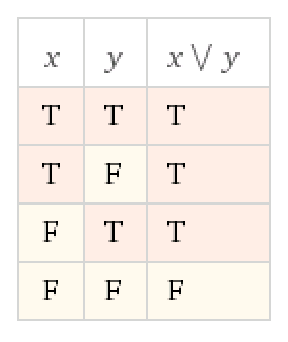
\includegraphics[scale=0.7]{images/eq_logic_or}
        \caption{Logical OR in CNF}
    \end{subfigure}
    \quad
    \begin{subfigure}[b]{0.5\textwidth}
        \centering
        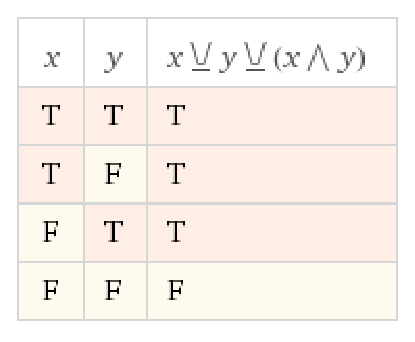
\includegraphics[scale=0.7]{images/eq_logic_or_anf}
        \caption{Logical OR in ANF}
    \end{subfigure}
	\caption{Truth tables for logical OR}
	\label{fig:eq_logic_or}
\end{figure}


\subsection{Bit permutations}

Consider simple $4$-bit permutation that needs to be defined by equations
system (figure~\ref{fig:eq_permutation}). After matching each bit to certain
variable one could obtain the corresponding equations system.
\begin{equation}
\label{eqn:eq_permutation_expl}
\left\{
	\begin{array}{ll}
        y_0 = x_3; \\
        y_1 = x_2; \\
        y_2 = x_1; \\
        y_3 = x_0. \\
	\end{array} \right.
\end{equation}
Then equations (\ref{eqn:eq_permutation_expl}) could be transformed to implicit
form to obtain the final polynomials:
\begin{equation}
\label{eqn:eq_permutation_impl}
\left\{
	\begin{array}{ll}
        y_0 \oplus x_3 = 0; \\
        y_1 \oplus x_2 = 0; \\
        y_2 \oplus x_1 = 0; \\
        y_3 \oplus x_0 = 0. \\
	\end{array} \right.
\end{equation}
So the given $4$-bit permutation has been defined by $4$ equations in $8$
variables.  Such solution is simple but unfortunately introduces more variables
than equations which may lead to underdefined and therefore unsolvable system.
However more efficient approach exists. Since there is no multiplication in this
transformation that could increase equations degree and the variables are only
renamed, they may be just reordered for the following transformation to receive
correct values. That way no additional equations or variables are introduced at
all.

Any cyclic bit shift is just a special case of ordered permutation and is
defined similarly.

\begin{figure}[htbp]
	\centering
    % Graphic for TeX using PGF
% Title: /home/zoresvit/devel/texmf/dstu-3008-95/images/eq_permutation.dia
% Creator: Dia v0.97.2
% CreationDate: Mon Jun  3 02:38:01 2013
% For: zoresvit
% \usepackage{tikz}
% The following commands are not supported in PSTricks at present
% We define them conditionally, so when they are implemented,
% this pgf file will use them.
\ifx\du\undefined
  \newlength{\du}
\fi
\setlength{\du}{15\unitlength}
\begin{tikzpicture}[scale=0.9,every node/.style={scale=1}]
\pgftransformxscale{1.000000}
\pgftransformyscale{-1.000000}
\definecolor{dialinecolor}{rgb}{0.000000, 0.000000, 0.000000}
\pgfsetstrokecolor{dialinecolor}
\definecolor{dialinecolor}{rgb}{1.000000, 1.000000, 1.000000}
\pgfsetfillcolor{dialinecolor}
\pgfsetlinewidth{0.100000\du}
\pgfsetdash{}{0pt}
\pgfsetdash{}{0pt}
\pgfsetbuttcap
{
\definecolor{dialinecolor}{rgb}{0.000000, 0.000000, 0.000000}
\pgfsetfillcolor{dialinecolor}
% was here!!!
\definecolor{dialinecolor}{rgb}{0.000000, 0.000000, 0.000000}
\pgfsetstrokecolor{dialinecolor}
\draw (19.000000\du,5.000000\du)--(19.000000\du,6.000000\du);
}
\pgfsetlinewidth{0.100000\du}
\pgfsetdash{}{0pt}
\pgfsetdash{}{0pt}
\pgfsetbuttcap
{
\definecolor{dialinecolor}{rgb}{0.000000, 0.000000, 0.000000}
\pgfsetfillcolor{dialinecolor}
% was here!!!
\definecolor{dialinecolor}{rgb}{0.000000, 0.000000, 0.000000}
\pgfsetstrokecolor{dialinecolor}
\draw (24.000000\du,5.000000\du)--(24.000000\du,6.000000\du);
}
\pgfsetlinewidth{0.100000\du}
\pgfsetdash{}{0pt}
\pgfsetdash{}{0pt}
\pgfsetbuttcap
{
\definecolor{dialinecolor}{rgb}{0.000000, 0.000000, 0.000000}
\pgfsetfillcolor{dialinecolor}
% was here!!!
\definecolor{dialinecolor}{rgb}{0.000000, 0.000000, 0.000000}
\pgfsetstrokecolor{dialinecolor}
\draw (21.500000\du,5.000000\du)--(21.500000\du,6.000000\du);
}
\pgfsetlinewidth{0.100000\du}
\pgfsetdash{}{0pt}
\pgfsetdash{}{0pt}
\pgfsetbuttcap
{
\definecolor{dialinecolor}{rgb}{0.000000, 0.000000, 0.000000}
\pgfsetfillcolor{dialinecolor}
% was here!!!
\definecolor{dialinecolor}{rgb}{0.000000, 0.000000, 0.000000}
\pgfsetstrokecolor{dialinecolor}
\draw (26.500000\du,5.000000\du)--(26.500000\du,6.000000\du);
}
\pgfsetlinewidth{0.100000\du}
\pgfsetdash{}{0pt}
\pgfsetdash{}{0pt}
\pgfsetbuttcap
{
\definecolor{dialinecolor}{rgb}{0.000000, 0.000000, 0.000000}
\pgfsetfillcolor{dialinecolor}
% was here!!!
\definecolor{dialinecolor}{rgb}{0.000000, 0.000000, 0.000000}
\pgfsetstrokecolor{dialinecolor}
\draw (19.000000\du,10.000000\du)--(19.000000\du,11.000000\du);
}
\pgfsetlinewidth{0.100000\du}
\pgfsetdash{}{0pt}
\pgfsetdash{}{0pt}
\pgfsetbuttcap
{
\definecolor{dialinecolor}{rgb}{0.000000, 0.000000, 0.000000}
\pgfsetfillcolor{dialinecolor}
% was here!!!
\definecolor{dialinecolor}{rgb}{0.000000, 0.000000, 0.000000}
\pgfsetstrokecolor{dialinecolor}
\draw (24.000000\du,10.000000\du)--(24.000000\du,11.000000\du);
}
\pgfsetlinewidth{0.100000\du}
\pgfsetdash{}{0pt}
\pgfsetdash{}{0pt}
\pgfsetbuttcap
{
\definecolor{dialinecolor}{rgb}{0.000000, 0.000000, 0.000000}
\pgfsetfillcolor{dialinecolor}
% was here!!!
\definecolor{dialinecolor}{rgb}{0.000000, 0.000000, 0.000000}
\pgfsetstrokecolor{dialinecolor}
\draw (21.500000\du,10.000000\du)--(21.500000\du,11.000000\du);
}
\pgfsetlinewidth{0.100000\du}
\pgfsetdash{}{0pt}
\pgfsetdash{}{0pt}
\pgfsetbuttcap
{
\definecolor{dialinecolor}{rgb}{0.000000, 0.000000, 0.000000}
\pgfsetfillcolor{dialinecolor}
% was here!!!
\definecolor{dialinecolor}{rgb}{0.000000, 0.000000, 0.000000}
\pgfsetstrokecolor{dialinecolor}
\draw (26.500000\du,10.000000\du)--(26.500000\du,11.000000\du);
}
\pgfsetlinewidth{0.100000\du}
\pgfsetdash{}{0pt}
\pgfsetdash{}{0pt}
\pgfsetbuttcap
{
\definecolor{dialinecolor}{rgb}{0.000000, 0.000000, 0.000000}
\pgfsetfillcolor{dialinecolor}
% was here!!!
\definecolor{dialinecolor}{rgb}{0.000000, 0.000000, 0.000000}
\pgfsetstrokecolor{dialinecolor}
\draw (21.500000\du,6.000000\du)--(26.500000\du,10.000000\du);
}
\pgfsetlinewidth{0.100000\du}
\pgfsetdash{}{0pt}
\pgfsetdash{}{0pt}
\pgfsetbuttcap
{
\definecolor{dialinecolor}{rgb}{0.000000, 0.000000, 0.000000}
\pgfsetfillcolor{dialinecolor}
% was here!!!
\definecolor{dialinecolor}{rgb}{0.000000, 0.000000, 0.000000}
\pgfsetstrokecolor{dialinecolor}
\draw (19.000000\du,6.000000\du)--(24.000000\du,10.000000\du);
}
\pgfsetlinewidth{0.100000\du}
\pgfsetdash{}{0pt}
\pgfsetdash{}{0pt}
\pgfsetbuttcap
{
\definecolor{dialinecolor}{rgb}{0.000000, 0.000000, 0.000000}
\pgfsetfillcolor{dialinecolor}
% was here!!!
\definecolor{dialinecolor}{rgb}{0.000000, 0.000000, 0.000000}
\pgfsetstrokecolor{dialinecolor}
\draw (24.000000\du,6.000000\du)--(21.500000\du,10.000000\du);
}
\pgfsetlinewidth{0.100000\du}
\pgfsetdash{}{0pt}
\pgfsetdash{}{0pt}
\pgfsetbuttcap
{
\definecolor{dialinecolor}{rgb}{0.000000, 0.000000, 0.000000}
\pgfsetfillcolor{dialinecolor}
% was here!!!
\definecolor{dialinecolor}{rgb}{0.000000, 0.000000, 0.000000}
\pgfsetstrokecolor{dialinecolor}
\draw (26.500000\du,6.000000\du)--(19.000000\du,10.000000\du);
}
% setfont left to latex
\definecolor{dialinecolor}{rgb}{0.000000, 0.000000, 0.000000}
\pgfsetstrokecolor{dialinecolor}
\node[anchor=west] at (18.000000\du,4.500000\du){$x_0$};
% setfont left to latex
\definecolor{dialinecolor}{rgb}{0.000000, 0.000000, 0.000000}
\pgfsetstrokecolor{dialinecolor}
\node[anchor=west] at (20.500000\du,4.500000\du){$x_1$};
% setfont left to latex
\definecolor{dialinecolor}{rgb}{0.000000, 0.000000, 0.000000}
\pgfsetstrokecolor{dialinecolor}
\node[anchor=west] at (23.000000\du,4.500000\du){$x_2$};
% setfont left to latex
\definecolor{dialinecolor}{rgb}{0.000000, 0.000000, 0.000000}
\pgfsetstrokecolor{dialinecolor}
\node[anchor=west] at (26.000000\du,4.500000\du){$x_3$};
% setfont left to latex
\definecolor{dialinecolor}{rgb}{0.000000, 0.000000, 0.000000}
\pgfsetstrokecolor{dialinecolor}
\node[anchor=west] at (18.000000\du,12.000000\du){$y_0$};
% setfont left to latex
\definecolor{dialinecolor}{rgb}{0.000000, 0.000000, 0.000000}
\pgfsetstrokecolor{dialinecolor}
\node[anchor=west] at (20.500000\du,12.000000\du){$y_1$};
% setfont left to latex
\definecolor{dialinecolor}{rgb}{0.000000, 0.000000, 0.000000}
\pgfsetstrokecolor{dialinecolor}
\node[anchor=west] at (23.000000\du,12.000000\du){$y_2$};
% setfont left to latex
\definecolor{dialinecolor}{rgb}{0.000000, 0.000000, 0.000000}
\pgfsetstrokecolor{dialinecolor}
\node[anchor=west] at (26.000000\du,12.000000\du){$y_3$};
\end{tikzpicture}

	\caption{$4$-bit permutation}
	\label{fig:eq_permutation}
\end{figure}

\subsection{Modular addition}
\label{seq:key-add-eqn}

During the Ukrainian national public cryptographic competition the following
method for defining modular addition with equations system has been proposed
by the author of \textit{Labyrinth} block cipher.

Modular addition $R = X + Y$ of two $n$-bit numbers is defined as
\begin{equation}
\label{eqn:add}
X = (x_0, \hdots, x_{n-1}), \;
Y = (y_0, \hdots, y_{n-1}), \;
R = (r_0, \hdots, r_{n-1}),
\end{equation}

where $i$ --- is a bit number, so $x_i$ represents $i$-th bit of number $X$.
Then the addition on a bit level is defined as follows:
\begin{equation}
\label{eqn:trivial-mod-add}
r_i = x_i \oplus y_i \oplus c_{i-1} \enspace,
\end{equation}

where $c_i$ is a carry bit variable and is defined by \eqref{eqn:carry-bit}.
\begin{equation}
\label{eqn:carry-bit}
c_i = r_{i+1} \oplus x_{i+1} \oplus y_{i+1} \enspace.
\end{equation}
The goal is to get null space equations for every addition bit without
explicitly using the carry variable. It turns out that for addition bits
$0 < i < (n - 1)$ three implicit equations may be defined:
\begin{equation}
\label{eqn:add-with-carry}
\left\{
	\begin{array}{ll}
        (x_i \oplus r_i) (x_i \oplus c_i) = 0; \\
        (y_i \oplus r_i) (y_i \oplus c_i) = 0; \\
        (x_i \oplus y_i) \cdot r_i \oplus x_i y_i \oplus x_i \oplus y_i \oplus c_i = 0.
	\end{array} \right.
\end{equation}
The final equation system that defines every addition bit may be extracted
from~\eqref{eqn:add-with-carry} by substituting every $c_i$ variable according
to~\ref{eqn:carry-bit}:
\begin{equation}
\label{eqn:mod-add}
\left\{
	\begin{array}{ll}
        x_i \oplus x_i r_i \oplus x_i r_{i+1} \oplus x_i x_{i+1} \oplus x_i y_{i+1} \oplus r_i r_{i+1} \oplus r_i x_{i+1} \oplus r_i y_{i+1} = 0; \\
        y_i \oplus y_i r_i \oplus y_i r_{i+1} \oplus y_i x_{i+1} \oplus y_i y_{i+1} \oplus r_i r_{i+1} \oplus r_i x_{i+1} \oplus r_i y_{i+1} = 0; \\
        x_i r_i \oplus y_i r_i \oplus x_i y_i \oplus x_i \oplus y_i \oplus r_{i+1} \oplus x_{i+1} \oplus y_{i+1} = 0.
	\end{array} \right.
\end{equation}
Thereby a single addition bit is defined by three equations of degree 2 each
containing $12$ quadratic terms. Even though the equations in
\eqref{eqn:mod-add} fully describe $n$-bit modular addition, adding a
redundant equation $r_0 = x_0 + y_0$ for the very first bit was found to give
crucial increase on system solving performance.


\subsection{S-boxes}

An arbitrary S-box is fully defined by equations of degree 2 that can be
obtained by finding null space equations as described in~\cite{kleiman:xsl}.

Consider the S-box $(7, 6, 0, 4, 2, 5, 1, 3)$ for example. To find
corresponding null space equations the following matrix $8 \times 22$ is
constructed.  Each row contains the values of all possible $22$ monomials for
each of $8$ possible inputs for variables $\{x_0, x_1, x_2, x_3\}$.
\begin{equation}
    \label{eqn:sbox-matr}
    \left(
    \begin{array}{lllllllll}
        1 &\quad 1 &\quad 1 &\quad 1 &\quad 1 &\quad 1 &\quad 1 &\quad 1 &\quad 1       \\[-1ex]
        0 &\quad 0 &\quad 0 &\quad 0 &\quad 1 &\quad 1 &\quad 1 &\quad 1 &\quad x_0     \\[-1ex]
        0 &\quad 0 &\quad 1 &\quad 1 &\quad 0 &\quad 0 &\quad 1 &\quad 1 &\quad x_1     \\[-1ex]
        0 &\quad 1 &\quad 0 &\quad 1 &\quad 0 &\quad 1 &\quad 0 &\quad 1 &\quad x_2     \\[-1ex]
        1 &\quad 1 &\quad 0 &\quad 1 &\quad 0 &\quad 1 &\quad 0 &\quad 0 &\quad y_0     \\[-1ex]
        1 &\quad 1 &\quad 0 &\quad 0 &\quad 1 &\quad 0 &\quad 0 &\quad 1 &\quad y_1     \\[-1ex]
        1 &\quad 0 &\quad 0 &\quad 0 &\quad 0 &\quad 1 &\quad 1 &\quad 1 &\quad y_2     \\[-1ex]
        0 &\quad 0 &\quad 0 &\quad 0 &\quad 0 &\quad 0 &\quad 1 &\quad 1 &\quad x_0 x_1 \\[-1ex]
        0 &\quad 0 &\quad 0 &\quad 0 &\quad 0 &\quad 1 &\quad 0 &\quad 1 &\quad x_0 x_2 \\[-1ex]
        0 &\quad 0 &\quad 0 &\quad 0 &\quad 0 &\quad 1 &\quad 0 &\quad 0 &\quad x_0 y_0 \\[-1ex]
        0 &\quad 0 &\quad 0 &\quad 0 &\quad 1 &\quad 0 &\quad 0 &\quad 1 &\quad x_0 y_1 \\[-1ex]
        0 &\quad 0 &\quad 0 &\quad 0 &\quad 0 &\quad 1 &\quad 1 &\quad 1 &\quad x_0 y_2 \\[-1ex]
        0 &\quad 0 &\quad 0 &\quad 1 &\quad 0 &\quad 0 &\quad 0 &\quad 1 &\quad x_1 x_2 \\[-1ex]
        0 &\quad 0 &\quad 0 &\quad 1 &\quad 0 &\quad 0 &\quad 0 &\quad 0 &\quad x_1 y_0 \\[-1ex]
        0 &\quad 0 &\quad 0 &\quad 0 &\quad 0 &\quad 0 &\quad 0 &\quad 1 &\quad x_1 y_1 \\[-1ex]
        0 &\quad 0 &\quad 0 &\quad 0 &\quad 0 &\quad 0 &\quad 1 &\quad 1 &\quad x_1 y_2 \\[-1ex]
        0 &\quad 1 &\quad 0 &\quad 1 &\quad 0 &\quad 1 &\quad 0 &\quad 0 &\quad x_2 y_0 \\[-1ex]
        0 &\quad 1 &\quad 0 &\quad 0 &\quad 0 &\quad 0 &\quad 0 &\quad 1 &\quad x_2 y_1 \\[-1ex]
        0 &\quad 0 &\quad 0 &\quad 0 &\quad 0 &\quad 1 &\quad 0 &\quad 1 &\quad x_2 y_2 \\[-1ex]
        1 &\quad 1 &\quad 0 &\quad 0 &\quad 0 &\quad 0 &\quad 0 &\quad 0 &\quad y_0 y_1 \\[-1ex]
        1 &\quad 0 &\quad 0 &\quad 0 &\quad 0 &\quad 1 &\quad 0 &\quad 0 &\quad y_0 y_2 \\[-1ex]
        1 &\quad 0 &\quad 0 &\quad 0 &\quad 0 &\quad 0 &\quad 0 &\quad 1 &\quad y_1 y_2
    \end{array} \right)
\end{equation}
The null space equations are then obtained by applying Gaussian elimination to
the matrix.

\begin{equation}
    \label{eqn:sbox-equations}
    \left(
    \begin{array}{llllllllr}
        1 & 0 & 0 & 0 & 0 & 0 & 0 & 0 & x_0 y_0+ x_1+ x_2+ y_0+ y_1+ 1              \\
        0 & 1 & 0 & 0 & 0 & 0 & 0 & 0 & x_0 y_0+ x_0+ x_1+ y_2+ 1                   \\
        0 & 0 & 1 & 0 & 0 & 0 & 0 & 0 & x_0 y_0+ x_0+ y_0+ 1                        \\
        0 & 0 & 0 & 1 & 0 & 0 & 0 & 0 & x_0 y_0+ x_0+ x_2+ y_1+ y_2                 \\
        0 & 0 & 0 & 0 & 1 & 0 & 0 & 0 & x_0 y_0+ x_0+ x_1+ x_2+ y_0+ y_1+ y_2+ 1    \\
        0 & 0 & 0 & 0 & 0 & 1 & 0 & 0 & x_0 y_0                                     \\
        0 & 0 & 0 & 0 & 0 & 0 & 1 & 0 & x_0 y_0+ x_2+ y_0+ y_2                      \\
        0 & 0 & 0 & 0 & 0 & 0 & 0 & 1 & x_0 y_0+ x_1+ y_1+ 1                        \\
        0 & 0 & 0 & 0 & 0 & 0 & 0 & 0 & x_0 x_2+ x_1+ y_1+ 1                        \\
        0 & 0 & 0 & 0 & 0 & 0 & 0 & 0 & x_0 x_1+ x_1+ x_2+ y_0+ y_1+ y_2+ 1         \\
        0 & 0 & 0 & 0 & 0 & 0 & 0 & 0 & x_0 y_1+ x_0+ x_2+ y_0+ y_2                 \\
        0 & 0 & 0 & 0 & 0 & 0 & 0 & 0 & x_0 y_0+ x_0y_2+ x_1+ x_2+ y_0+ y_1+ y_2+ 1 \\
        0 & 0 & 0 & 0 & 0 & 0 & 0 & 0 & x_1 x_2+ x_0+ x_1+ x_2+ y_2+ 1              \\
        0 & 0 & 0 & 0 & 0 & 0 & 0 & 0 & x_0 y_0+ x_1y_0+ x_0+ x_2+ y_1+ y_2         \\
        0 & 0 & 0 & 0 & 0 & 0 & 0 & 0 & x_0 y_0+ x_1y_1+ x_1+ y_1+ 1                \\
        0 & 0 & 0 & 0 & 0 & 0 & 0 & 0 & x_1 y_2+ x_1+ x_2+ y_0+ y_1+ y_2+ 1         \\
        0 & 0 & 0 & 0 & 0 & 0 & 0 & 0 & x_0 y_0+ x_2y_0+ x_1+ x_2+ y_1+ 1           \\
        0 & 0 & 0 & 0 & 0 & 0 & 0 & 0 & x_2 y_1+ x_0+ y_1+ y_2                      \\
        0 & 0 & 0 & 0 & 0 & 0 & 0 & 0 & x_2 y_2+ x_1+ y_1+ 1                        \\
        0 & 0 & 0 & 0 & 0 & 0 & 0 & 0 & y_0 y_1+ x_0+ x_2+ y_0+ y_1+ y_2            \\
        0 & 0 & 0 & 0 & 0 & 0 & 0 & 0 & y_0 y_2+ x_1+ x_2+ y_0+ y_1+ 1              \\
        0 & 0 & 0 & 0 & 0 & 0 & 0 & 0 & y_1 y_2+ x_2+ y_0
    \end{array} \right)
\end{equation}
This yields to $14$ equations that fully describe the S-box transformations.

\subsection{Feistel network}

Using the described methods of constructing algebraic equations for widely used
cryptographic transformations it is straightforward to define generic Feistel
network with polynomial equations system.

Consider a Feistel network on figure~\ref{fig:eq_feistel}.
\begin{figure}[htbp]
	\centering
    % Graphic for TeX using PGF
% Title: /home/zoresvit/devel/texmf/dstu-3008-95/images/feistel.dia
% Creator: Dia v0.97.2
% CreationDate: Tue Jun  4 00:25:14 2013
% For: zoresvit
% \usepackage{tikz}
% The following commands are not supported in PSTricks at present
% We define them conditionally, so when they are implemented,
% this pgf file will use them.
\ifx\du\undefined
  \newlength{\du}
\fi
\setlength{\du}{15\unitlength}
\begin{tikzpicture}[scale=0.6,every node/.style={scale=0.6}]
\pgftransformxscale{1.000000}
\pgftransformyscale{-1.000000}
\definecolor{dialinecolor}{rgb}{0.000000, 0.000000, 0.000000}
\pgfsetstrokecolor{dialinecolor}
\definecolor{dialinecolor}{rgb}{1.000000, 1.000000, 1.000000}
\pgfsetfillcolor{dialinecolor}
\definecolor{dialinecolor}{rgb}{1.000000, 1.000000, 1.000000}
\pgfsetfillcolor{dialinecolor}
\fill (16.000000\du,2.000000\du)--(16.000000\du,3.900000\du)--(28.000000\du,3.900000\du)--(28.000000\du,2.000000\du)--cycle;
\pgfsetlinewidth{0.100000\du}
\pgfsetdash{}{0pt}
\pgfsetdash{}{0pt}
\pgfsetmiterjoin
\definecolor{dialinecolor}{rgb}{0.000000, 0.000000, 0.000000}
\pgfsetstrokecolor{dialinecolor}
\draw (16.000000\du,2.000000\du)--(16.000000\du,3.900000\du)--(28.000000\du,3.900000\du)--(28.000000\du,2.000000\du)--cycle;
% setfont left to latex
\definecolor{dialinecolor}{rgb}{0.000000, 0.000000, 0.000000}
\pgfsetstrokecolor{dialinecolor}
\node at (22.000000\du,3.145000\du){INPUT};
\definecolor{dialinecolor}{rgb}{1.000000, 1.000000, 1.000000}
\pgfsetfillcolor{dialinecolor}
\fill (16.000000\du,12.000000\du)--(16.000000\du,13.900000\du)--(28.000000\du,13.900000\du)--(28.000000\du,12.000000\du)--cycle;
\pgfsetlinewidth{0.100000\du}
\pgfsetdash{}{0pt}
\pgfsetdash{}{0pt}
\pgfsetmiterjoin
\definecolor{dialinecolor}{rgb}{0.000000, 0.000000, 0.000000}
\pgfsetstrokecolor{dialinecolor}
\draw (16.000000\du,12.000000\du)--(16.000000\du,13.900000\du)--(28.000000\du,13.900000\du)--(28.000000\du,12.000000\du)--cycle;
% setfont left to latex
\definecolor{dialinecolor}{rgb}{0.000000, 0.000000, 0.000000}
\pgfsetstrokecolor{dialinecolor}
\node at (22.000000\du,13.145000\du){OUTPUT};
\definecolor{dialinecolor}{rgb}{1.000000, 1.000000, 1.000000}
\pgfsetfillcolor{dialinecolor}
\fill (30.000000\du,2.000000\du)--(30.000000\du,3.900000\du)--(36.000000\du,3.900000\du)--(36.000000\du,2.000000\du)--cycle;
\pgfsetlinewidth{0.100000\du}
\pgfsetdash{}{0pt}
\pgfsetdash{}{0pt}
\pgfsetmiterjoin
\definecolor{dialinecolor}{rgb}{0.000000, 0.000000, 0.000000}
\pgfsetstrokecolor{dialinecolor}
\draw (30.000000\du,2.000000\du)--(30.000000\du,3.900000\du)--(36.000000\du,3.900000\du)--(36.000000\du,2.000000\du)--cycle;
% setfont left to latex
\definecolor{dialinecolor}{rgb}{0.000000, 0.000000, 0.000000}
\pgfsetstrokecolor{dialinecolor}
\node at (33.000000\du,3.145000\du){SUBKEY};
\pgfsetlinewidth{0.100000\du}
\pgfsetdash{}{0pt}
\pgfsetdash{}{0pt}
\pgfsetbuttcap
{
\definecolor{dialinecolor}{rgb}{0.000000, 0.000000, 0.000000}
\pgfsetfillcolor{dialinecolor}
% was here!!!
\definecolor{dialinecolor}{rgb}{0.000000, 0.000000, 0.000000}
\pgfsetstrokecolor{dialinecolor}
\draw (26.500000\du,4.500000\du)--(26.500000\du,8.000000\du);
}
\pgfsetlinewidth{0.100000\du}
\pgfsetdash{}{0pt}
\pgfsetdash{}{0pt}
\pgfsetmiterjoin
\pgfsetbuttcap
{
\definecolor{dialinecolor}{rgb}{0.000000, 0.000000, 0.000000}
\pgfsetfillcolor{dialinecolor}
% was here!!!
{\pgfsetcornersarced{\pgfpoint{0.000000\du}{0.000000\du}}\definecolor{dialinecolor}{rgb}{0.000000, 0.000000, 0.000000}
\pgfsetstrokecolor{dialinecolor}
\draw (33.000000\du,3.900000\du)--(33.000000\du,5.264262\du)--(26.773042\du,5.264262\du)--(26.773042\du,5.269734\du);
}}
% setfont left to latex
\definecolor{dialinecolor}{rgb}{0.000000, 0.000000, 0.000000}
\pgfsetstrokecolor{dialinecolor}
\node[anchor=west] at (16.000000\du,1.500000\du){0};
% setfont left to latex
\definecolor{dialinecolor}{rgb}{0.000000, 0.000000, 0.000000}
\pgfsetstrokecolor{dialinecolor}
\node[anchor=west] at (21.000000\du,1.500000\du){31  32};
% setfont left to latex
\definecolor{dialinecolor}{rgb}{0.000000, 0.000000, 0.000000}
\pgfsetstrokecolor{dialinecolor}
\node[anchor=west] at (27.000000\du,1.500000\du){63};
% setfont left to latex
\definecolor{dialinecolor}{rgb}{0.000000, 0.000000, 0.000000}
\pgfsetstrokecolor{dialinecolor}
\node[anchor=west] at (30.000000\du,1.500000\du){0};
% setfont left to latex
\definecolor{dialinecolor}{rgb}{0.000000, 0.000000, 0.000000}
\pgfsetstrokecolor{dialinecolor}
\node[anchor=west] at (35.500000\du,1.500000\du){31};
\pgfsetlinewidth{0.100000\du}
\pgfsetdash{}{0pt}
\pgfsetdash{}{0pt}
\pgfsetbuttcap
{
\definecolor{dialinecolor}{rgb}{0.000000, 0.000000, 0.000000}
\pgfsetfillcolor{dialinecolor}
% was here!!!
\definecolor{dialinecolor}{rgb}{0.000000, 0.000000, 0.000000}
\pgfsetstrokecolor{dialinecolor}
\pgfpathmoveto{\pgfpoint{26.770270\du}{5.309030\du}}
\pgfpatharc{360}{181}{0.300000\du and 0.300000\du}
\pgfusepath{stroke}
}
% setfont left to latex
\definecolor{dialinecolor}{rgb}{0.000000, 0.000000, 0.000000}
\pgfsetstrokecolor{dialinecolor}
\node[anchor=west] at (30.000000\du,4.600000\du){$K_{0..32}$};
\pgfsetlinewidth{0.100000\du}
\pgfsetdash{}{0pt}
\pgfsetdash{}{0pt}
\pgfsetbuttcap
{
\definecolor{dialinecolor}{rgb}{0.000000, 0.000000, 0.000000}
\pgfsetfillcolor{dialinecolor}
% was here!!!
\definecolor{dialinecolor}{rgb}{0.000000, 0.000000, 0.000000}
\pgfsetstrokecolor{dialinecolor}
\draw (26.500000\du,8.000000\du)--(17.500000\du,9.500000\du);
}
\pgfsetlinewidth{0.100000\du}
\pgfsetdash{}{0pt}
\pgfsetdash{}{0pt}
\pgfsetmiterjoin
\pgfsetbuttcap
{
\definecolor{dialinecolor}{rgb}{0.000000, 0.000000, 0.000000}
\pgfsetfillcolor{dialinecolor}
% was here!!!
\definecolor{dialinecolor}{rgb}{0.000000, 0.000000, 0.000000}
\pgfsetstrokecolor{dialinecolor}
\pgfpathmoveto{\pgfpoint{26.500000\du}{4.500000\du}}
\pgfpathcurveto{\pgfpoint{26.500000\du}{3.900000\du}}{\pgfpoint{22.000000\du}{4.500000\du}}{\pgfpoint{22.000000\du}{3.900000\du}}
\pgfusepath{stroke}
}
\pgfsetlinewidth{0.100000\du}
\pgfsetdash{}{0pt}
\pgfsetdash{}{0pt}
\pgfsetmiterjoin
\pgfsetbuttcap
{
\definecolor{dialinecolor}{rgb}{0.000000, 0.000000, 0.000000}
\pgfsetfillcolor{dialinecolor}
% was here!!!
\definecolor{dialinecolor}{rgb}{0.000000, 0.000000, 0.000000}
\pgfsetstrokecolor{dialinecolor}
\pgfpathmoveto{\pgfpoint{26.500000\du}{4.500000\du}}
\pgfpathcurveto{\pgfpoint{26.500000\du}{4.100000\du}}{\pgfpoint{28.000000\du}{4.600000\du}}{\pgfpoint{28.000000\du}{4.000000\du}}
\pgfusepath{stroke}
}
\pgfsetlinewidth{0.100000\du}
\pgfsetdash{}{0pt}
\pgfsetdash{}{0pt}
\pgfsetmiterjoin
\pgfsetbuttcap
{
\definecolor{dialinecolor}{rgb}{0.000000, 0.000000, 0.000000}
\pgfsetfillcolor{dialinecolor}
% was here!!!
\definecolor{dialinecolor}{rgb}{0.000000, 0.000000, 0.000000}
\pgfsetstrokecolor{dialinecolor}
\pgfpathmoveto{\pgfpoint{17.500000\du}{11.500000\du}}
\pgfpathcurveto{\pgfpoint{17.500000\du}{11.880000\du}}{\pgfpoint{16.000000\du}{11.500000\du}}{\pgfpoint{16.000000\du}{12.000000\du}}
\pgfusepath{stroke}
}
\pgfsetlinewidth{0.100000\du}
\pgfsetdash{}{0pt}
\pgfsetdash{}{0pt}
\pgfsetmiterjoin
\pgfsetbuttcap
{
\definecolor{dialinecolor}{rgb}{0.000000, 0.000000, 0.000000}
\pgfsetfillcolor{dialinecolor}
% was here!!!
\definecolor{dialinecolor}{rgb}{0.000000, 0.000000, 0.000000}
\pgfsetstrokecolor{dialinecolor}
\pgfpathmoveto{\pgfpoint{17.500000\du}{11.500000\du}}
\pgfpathcurveto{\pgfpoint{17.500000\du}{12.100000\du}}{\pgfpoint{22.000000\du}{11.300000\du}}{\pgfpoint{22.000000\du}{12.000000\du}}
\pgfusepath{stroke}
}
\pgfsetlinewidth{0.100000\du}
\pgfsetdash{}{0pt}
\pgfsetdash{}{0pt}
\pgfsetbuttcap
{
\definecolor{dialinecolor}{rgb}{0.000000, 0.000000, 0.000000}
\pgfsetfillcolor{dialinecolor}
% was here!!!
\pgfsetarrowsend{stealth}
\definecolor{dialinecolor}{rgb}{0.000000, 0.000000, 0.000000}
\pgfsetstrokecolor{dialinecolor}
\draw (17.500000\du,9.500000\du)--(17.500000\du,11.500000\du);
}
\definecolor{dialinecolor}{rgb}{1.000000, 1.000000, 1.000000}
\pgfsetfillcolor{dialinecolor}
\fill (21.679508\du,5.922890\du)--(21.679508\du,8.081223\du)--(23.769502\du,8.081223\du)--(23.769502\du,5.922890\du)--cycle;
\pgfsetlinewidth{0.100000\du}
\pgfsetdash{}{0pt}
\pgfsetdash{}{0pt}
\pgfsetmiterjoin
\definecolor{dialinecolor}{rgb}{0.000000, 0.000000, 0.000000}
\pgfsetstrokecolor{dialinecolor}
\draw (21.679508\du,5.922890\du)--(21.679508\du,8.081223\du)--(23.769502\du,8.081223\du)--(23.769502\du,5.922890\du)--cycle;
% setfont left to latex
\definecolor{dialinecolor}{rgb}{0.000000, 0.000000, 0.000000}
\pgfsetstrokecolor{dialinecolor}
\node at (22.724505\du,7.260390\du){F};
\pgfsetlinewidth{0.100000\du}
\pgfsetdash{}{0pt}
\pgfsetdash{}{0pt}
\pgfsetmiterjoin
\pgfsetbuttcap
{
\definecolor{dialinecolor}{rgb}{0.000000, 0.000000, 0.000000}
\pgfsetfillcolor{dialinecolor}
% was here!!!
\pgfsetarrowsend{stealth}
{\pgfsetcornersarced{\pgfpoint{0.000000\du}{0.000000\du}}\definecolor{dialinecolor}{rgb}{0.000000, 0.000000, 0.000000}
\pgfsetstrokecolor{dialinecolor}
\draw (26.137119\du,5.301268\du)--(26.137119\du,5.262830\du)--(22.724505\du,5.262830\du)--(22.724505\du,5.922890\du);
}}
\pgfsetlinewidth{0.100000\du}
\pgfsetdash{}{0pt}
\pgfsetdash{}{0pt}
\pgfsetbuttcap
{
\definecolor{dialinecolor}{rgb}{0.000000, 0.000000, 0.000000}
\pgfsetfillcolor{dialinecolor}
% was here!!!
\pgfsetarrowsend{stealth}
\definecolor{dialinecolor}{rgb}{0.000000, 0.000000, 0.000000}
\pgfsetstrokecolor{dialinecolor}
\draw (26.484530\du,7.000000\du)--(23.769502\du,7.002057\du);
}
\pgfsetlinewidth{0.100000\du}
\pgfsetdash{}{0pt}
\pgfsetdash{}{0pt}
\pgfsetmiterjoin
\pgfsetbuttcap
{
\definecolor{dialinecolor}{rgb}{0.000000, 0.000000, 0.000000}
\pgfsetfillcolor{dialinecolor}
% was here!!!
\definecolor{dialinecolor}{rgb}{0.000000, 0.000000, 0.000000}
\pgfsetstrokecolor{dialinecolor}
\pgfpathmoveto{\pgfpoint{17.500000\du}{4.500000\du}}
\pgfpathcurveto{\pgfpoint{17.500000\du}{4.100000\du}}{\pgfpoint{16.000000\du}{4.600000\du}}{\pgfpoint{16.000000\du}{4.000000\du}}
\pgfusepath{stroke}
}
\pgfsetlinewidth{0.100000\du}
\pgfsetdash{}{0pt}
\pgfsetdash{}{0pt}
\pgfsetmiterjoin
\pgfsetbuttcap
{
\definecolor{dialinecolor}{rgb}{0.000000, 0.000000, 0.000000}
\pgfsetfillcolor{dialinecolor}
% was here!!!
\definecolor{dialinecolor}{rgb}{0.000000, 0.000000, 0.000000}
\pgfsetstrokecolor{dialinecolor}
\pgfpathmoveto{\pgfpoint{17.500000\du}{4.500000\du}}
\pgfpathcurveto{\pgfpoint{17.500000\du}{4.000000\du}}{\pgfpoint{22.000000\du}{4.500000\du}}{\pgfpoint{22.000000\du}{3.900000\du}}
\pgfusepath{stroke}
}
\pgfsetlinewidth{0.100000\du}
\pgfsetdash{}{0pt}
\pgfsetdash{}{0pt}
\pgfsetbuttcap
\pgfsetmiterjoin
\pgfsetlinewidth{0.100000\du}
\pgfsetbuttcap
\pgfsetmiterjoin
\pgfsetdash{}{0pt}
\definecolor{dialinecolor}{rgb}{1.000000, 1.000000, 1.000000}
\pgfsetfillcolor{dialinecolor}
\pgfpathellipse{\pgfpoint{17.500000\du}{7.000000\du}}{\pgfpoint{0.500000\du}{0\du}}{\pgfpoint{0\du}{0.500000\du}}
\pgfusepath{fill}
\definecolor{dialinecolor}{rgb}{0.000000, 0.000000, 0.000000}
\pgfsetstrokecolor{dialinecolor}
\pgfpathellipse{\pgfpoint{17.500000\du}{7.000000\du}}{\pgfpoint{0.500000\du}{0\du}}{\pgfpoint{0\du}{0.500000\du}}
\pgfusepath{stroke}
\pgfsetbuttcap
\pgfsetmiterjoin
\pgfsetdash{}{0pt}
\definecolor{dialinecolor}{rgb}{0.000000, 0.000000, 0.000000}
\pgfsetstrokecolor{dialinecolor}
\draw (17.500000\du,6.500000\du)--(17.500000\du,7.500000\du);
\pgfsetbuttcap
\pgfsetmiterjoin
\pgfsetdash{}{0pt}
\definecolor{dialinecolor}{rgb}{0.000000, 0.000000, 0.000000}
\pgfsetstrokecolor{dialinecolor}
\draw (17.000000\du,7.000000\du)--(18.000000\du,7.000000\du);
\pgfsetlinewidth{0.100000\du}
\pgfsetdash{}{0pt}
\pgfsetdash{}{0pt}
\pgfsetbuttcap
{
\definecolor{dialinecolor}{rgb}{0.000000, 0.000000, 0.000000}
\pgfsetfillcolor{dialinecolor}
% was here!!!
\pgfsetarrowsend{stealth}
\definecolor{dialinecolor}{rgb}{0.000000, 0.000000, 0.000000}
\pgfsetstrokecolor{dialinecolor}
\draw (21.679508\du,7.002057\du)--(18.000000\du,7.000000\du);
}
\pgfsetlinewidth{0.100000\du}
\pgfsetdash{}{0pt}
\pgfsetdash{}{0pt}
\pgfsetbuttcap
{
\definecolor{dialinecolor}{rgb}{0.000000, 0.000000, 0.000000}
\pgfsetfillcolor{dialinecolor}
% was here!!!
\definecolor{dialinecolor}{rgb}{0.000000, 0.000000, 0.000000}
\pgfsetstrokecolor{dialinecolor}
\draw (17.500000\du,4.500000\du)--(17.500000\du,6.500000\du);
}
\pgfsetlinewidth{0.100000\du}
\pgfsetdash{}{0pt}
\pgfsetdash{}{0pt}
\pgfsetbuttcap
{
\definecolor{dialinecolor}{rgb}{0.000000, 0.000000, 0.000000}
\pgfsetfillcolor{dialinecolor}
% was here!!!
\definecolor{dialinecolor}{rgb}{0.000000, 0.000000, 0.000000}
\pgfsetstrokecolor{dialinecolor}
\draw (17.500000\du,7.500000\du)--(17.500000\du,8.000000\du);
}
\pgfsetlinewidth{0.100000\du}
\pgfsetdash{}{0pt}
\pgfsetdash{}{0pt}
\pgfsetbuttcap
{
\definecolor{dialinecolor}{rgb}{0.000000, 0.000000, 0.000000}
\pgfsetfillcolor{dialinecolor}
% was here!!!
\definecolor{dialinecolor}{rgb}{0.000000, 0.000000, 0.000000}
\pgfsetstrokecolor{dialinecolor}
\draw (17.500000\du,8.000000\du)--(26.500000\du,9.500000\du);
}
\pgfsetlinewidth{0.100000\du}
\pgfsetdash{}{0pt}
\pgfsetdash{}{0pt}
\pgfsetmiterjoin
\pgfsetbuttcap
{
\definecolor{dialinecolor}{rgb}{0.000000, 0.000000, 0.000000}
\pgfsetfillcolor{dialinecolor}
% was here!!!
\definecolor{dialinecolor}{rgb}{0.000000, 0.000000, 0.000000}
\pgfsetstrokecolor{dialinecolor}
\pgfpathmoveto{\pgfpoint{26.500000\du}{11.500000\du}}
\pgfpathcurveto{\pgfpoint{26.500000\du}{12.000000\du}}{\pgfpoint{22.000000\du}{11.300000\du}}{\pgfpoint{22.000000\du}{12.000000\du}}
\pgfusepath{stroke}
}
\pgfsetlinewidth{0.100000\du}
\pgfsetdash{}{0pt}
\pgfsetdash{}{0pt}
\pgfsetmiterjoin
\pgfsetbuttcap
{
\definecolor{dialinecolor}{rgb}{0.000000, 0.000000, 0.000000}
\pgfsetfillcolor{dialinecolor}
% was here!!!
\definecolor{dialinecolor}{rgb}{0.000000, 0.000000, 0.000000}
\pgfsetstrokecolor{dialinecolor}
\pgfpathmoveto{\pgfpoint{26.500000\du}{11.500000\du}}
\pgfpathcurveto{\pgfpoint{26.500000\du}{11.900000\du}}{\pgfpoint{28.000000\du}{11.400000\du}}{\pgfpoint{28.000000\du}{12.000000\du}}
\pgfusepath{stroke}
}
\pgfsetlinewidth{0.100000\du}
\pgfsetdash{}{0pt}
\pgfsetdash{}{0pt}
\pgfsetbuttcap
{
\definecolor{dialinecolor}{rgb}{0.000000, 0.000000, 0.000000}
\pgfsetfillcolor{dialinecolor}
% was here!!!
\pgfsetarrowsend{stealth}
\definecolor{dialinecolor}{rgb}{0.000000, 0.000000, 0.000000}
\pgfsetstrokecolor{dialinecolor}
\draw (26.500000\du,9.500000\du)--(26.500000\du,11.500000\du);
}
% setfont left to latex
\definecolor{dialinecolor}{rgb}{0.000000, 0.000000, 0.000000}
\pgfsetstrokecolor{dialinecolor}
\node[anchor=west] at (14.500000\du,5.400000\du){$X_{0..31}$};
% setfont left to latex
\definecolor{dialinecolor}{rgb}{0.000000, 0.000000, 0.000000}
\pgfsetstrokecolor{dialinecolor}
\node[anchor=west] at (26.500000\du,6.300000\du){$X_{32..63}$};
% setfont left to latex
\definecolor{dialinecolor}{rgb}{0.000000, 0.000000, 0.000000}
\pgfsetstrokecolor{dialinecolor}
\node[anchor=west] at (16.000000\du,14.772625\du){0};
% setfont left to latex
\definecolor{dialinecolor}{rgb}{0.000000, 0.000000, 0.000000}
\pgfsetstrokecolor{dialinecolor}
\node[anchor=west] at (21.000000\du,14.772625\du){31  32};
% setfont left to latex
\definecolor{dialinecolor}{rgb}{0.000000, 0.000000, 0.000000}
\pgfsetstrokecolor{dialinecolor}
\node[anchor=west] at (27.000000\du,14.772625\du){63};
% setfont left to latex
\definecolor{dialinecolor}{rgb}{0.000000, 0.000000, 0.000000}
\pgfsetstrokecolor{dialinecolor}
\node[anchor=west] at (18.500000\du,6.100000\du){$Z_{32..63}$};
% setfont left to latex
\definecolor{dialinecolor}{rgb}{0.000000, 0.000000, 0.000000}
\pgfsetstrokecolor{dialinecolor}
\node[anchor=west] at (23.500000\du,11.000000\du){$Y_{32..63}$};
% setfont left to latex
\definecolor{dialinecolor}{rgb}{0.000000, 0.000000, 0.000000}
\pgfsetstrokecolor{dialinecolor}
\node[anchor=west] at (18.000000\du,11.000000\du){$Y_{0..31}$};
\end{tikzpicture}

	\caption{Feistel network}
    \label{fig:eq_feistel}
\end{figure}
All input and output bits of the Festel network are considered to be unknown and
therefore are replaced with variables. Then going through each transformation
those variables are used for equations construction that are further assigned to
next variables for the following transformation. This example on
figure~\ref{fig:eq_feistel} demonstrates such process for single round of
Feistel network. The resulting number of equations and variables depends on
transformations used in $F$ function. For full-scale Feistel networks the
internal variables for each round must be distinct. This may be achieved by
prefixing variables names with current round number. However the output
variables of round $n$ are equal to input variables of adjacent round $n+1$ and
therefore are common.

Some transformations (like modular addition and S-boxes) increase the degree of
monomials. There are two possible ways of preventing the equations degree
growth: with preprocessing or post-processing. The preprocessing implies
introducing new variables before each transformation that contains
multiplication. Post-processing however decreases the degree of already
constructed equations until they become quadratic by applying the following
operation repeatedly:
\begin{equation}
\{m = w x y z\} \Rightarrow \{a = wx;\; b = yz;\; m = ab \}\enspace.
\end{equation}

Many ciphers based on Feistel networks (including the studied ones) use the key
that is larger than the block size. Therefore a single known plaintext and
ciphertext pair may not introduce enough information for recovering all the key
bits. In this case several systems of equations should be joined together. Such
systems share only the key variables (and variables for subkeys and key
scheduling if any) while the rest of variables are distinct. Then the plaintext
and ciphertext pairs obtained on the same key must be injected into the extended
system. The number of introduced known values for \mbox{plaintext/ciphertext}
variables must be equal to the unicity distance of the cipher.


\section{Methods for solving algebraic equation systems}

\subsection{Gr\"obner basis}
\label{sec:groebner}

Finding a Gr\"obner basis is equivalent to solving various problems concerning
polynomial systems~\cite{bard2009algebraic}. As Gaussian elimination method
solves linear equation systems, the Gr\"obner basis is designed to do the same
for non-linear polynomial systems.

In~\cite{Albrecht2006} the Gr\"obner basis is defined as following.

For a fixed monomial order a finite subset $G = \{g_0, \hdots, g_{m-1}\}$
of an ideal $\mathbb{I}$ is said to be a Gr\"obner basis if
\begin{equation}
    \label{eqn:groebner}
    \left< LT(g_0), \hdots, LT(g_{m-1}) \right> = \left< LT(I) \right> \enspace,
\end{equation}

where $LT$ denotes the leading term of a polynomial.

Notably the leading term of every polynomial from $\mathbb{I}$ is divisible by
the leading term of at least one polynomial from $\mathbb{G}$.

Gr\"obner basis has been successfully applied for attacking several ciphers,
including FLURRY and CURRY~\cite{Pyshkin2008:groebner} and even showed to be
more efficient than SAT solvers in algebraic attack on
Bivium~\cite{springerlink:10.1007/s11786-009-0016-7}.

Even though in most cases Gr\"obner basis method is not efficient enough for
attacking full-scale ciphers it is useful for exhausting more linearly
independent equations by applying it to some transformations (like S-boxes).

\subsection{SAT solvers}

Another approach to solving MQ problem is SAT\footnote{SAT is an abbreviation
denoting boolean satisfiability problem.} solvers that are used for
determining a set of variables that would satisfy a given boolean formula.

An efficient method of converting equation systems from the algebraic normal
form (ANF) to the conjunctive normal form (CNF) was proposed
in~\cite{cryptoeprint-2007-024}. After conversion the resulting system is
solved by a SAT solver of cryptanalyst's choice. SAT solvers also require less
memory and make it possible to solve problems infeasible for Gr\"obner basis
algorithms.

SAT solvers gained lots of attention lately since the problem of finding
solutions satisfying a given system of boolean equations is \mbox{NP-complete}
so developing a SAT solving algorithm running in polynomial time would help to
experimentally show equality of P and NP. So proving (or disapproving) the
equivalence of these two complexity classes would affect not only asymmetric
ciphers based on factorization problem as was though before, but any cipher that
may be efficiently described by an algebraic equations system.


\section{Summary}

In this chapter the methods for defining most widely used cryptographic
primitives with system of non-linear equations are described. The techniques of
obtaining equations for bit permutations, modular addition, some logical
operations and S-boxes should allow to construct full-scale non-linear equations
systems for most modern symmetric ciphers.

Also some most efficient methods for solving the constructed system of equations
are described. The software tools for computational algebra that provide needed
functionality are described in section~\ref{sec:implementation}. Reference
implementation for defining individual transformations with non-linear equations
and constructing full-scale system of equations is provided in
appendices~\ref{app:gost}-\ref{app:misty-solve}. A computational power of
low-end computer will not make it possible to perform an algebraic attack on
full-scale cipher but will allow to research algebraic properties of individual
transformations to make predictions for cipher security.


\chapter{Algebraic attack on \gost\ and \misty}


\section{Description of GOST~28147-89 cipher}
\label{sec:algebraic-gost}

Officially adopted in 1989 the GOST~28147 cipher has been developed in
former USSR and is now the encryption standard in most CIS countries.
For more than 20 years of cryptanalysis no efficient attack that would
significantly reduce the cipher security had been found.

GOST~28147-89 is a symmetric block cipher with a key length of 256 bits. It's
represented by a Feistel network of 32 rounds. The round function consists of
key addition modulo $2^{32}$, substitution layer represented by eight 4-bit
S-boxes, and a cyclic left shift by 11 bits (figure~\ref{fig:gost-round-func}).
S-boxes are not defined in the
original standard~\cite{GOST28147}. For some time they were considered to be
another secret parameter, but such approach caused more problems than gained
additional security. Use of different S-boxes set caused some cipher
implementations to be incompatible. Later all possible benefits of secret
substitution layer were scattered by introducing a method to recover all
unknown S-boxes in $2^{32}$ encryptions~\cite{saarinen1998:sboxes}.
\begin{figure}[htbp]
    \centering
    % Graphic for TeX using PGF
% Title: /home/zoresvit/Documents/diploma/bachelor-thesis/images/gost.dia
% Creator: Dia v0.97.1
% CreationDate: Wed May  9 22:47:17 2012
% For: zoresvit
% \usepackage{tikz}
% The following commands are not supported in PSTricks at present
% We define them conditionally, so when they are implemented,
% this pgf file will use them.
\ifx\du\undefined
  \newlength{\du}
\fi
\setlength{\du}{15\unitlength}
\begin{tikzpicture}[every node/.style={scale=0.8}]
\pgftransformxscale{1.000000}
\pgftransformyscale{-1.000000}
\definecolor{dialinecolor}{rgb}{0.000000, 0.000000, 0.000000}
\pgfsetstrokecolor{dialinecolor}
\definecolor{dialinecolor}{rgb}{1.000000, 1.000000, 1.000000}
\pgfsetfillcolor{dialinecolor}
\definecolor{dialinecolor}{rgb}{1.000000, 1.000000, 1.000000}
\pgfsetfillcolor{dialinecolor}
\fill (16.000000\du,2.000000\du)--(16.000000\du,4.000000\du)--(28.000000\du,4.000000\du)--(28.000000\du,2.000000\du)--cycle;
\pgfsetlinewidth{0.100000\du}
\pgfsetdash{}{0pt}
\pgfsetdash{}{0pt}
\pgfsetmiterjoin
\definecolor{dialinecolor}{rgb}{0.000000, 0.000000, 0.000000}
\pgfsetstrokecolor{dialinecolor}
\draw (16.000000\du,2.000000\du)--(16.000000\du,4.000000\du)--(28.000000\du,4.000000\du)--(28.000000\du,2.000000\du)--cycle;
% setfont left to latex
\definecolor{dialinecolor}{rgb}{0.000000, 0.000000, 0.000000}
\pgfsetstrokecolor{dialinecolor}
\node at (22.000000\du,3.000000\du){INPUT};
\definecolor{dialinecolor}{rgb}{1.000000, 1.000000, 1.000000}
\pgfsetfillcolor{dialinecolor}
\fill (16.000000\du,12.000000\du)--(16.000000\du,14.000000\du)--(28.000000\du,14.000000\du)--(28.000000\du,12.000000\du)--cycle;
\pgfsetlinewidth{0.100000\du}
\pgfsetdash{}{0pt}
\pgfsetdash{}{0pt}
\pgfsetmiterjoin
\definecolor{dialinecolor}{rgb}{0.000000, 0.000000, 0.000000}
\pgfsetstrokecolor{dialinecolor}
\draw (16.000000\du,12.000000\du)--(16.000000\du,14.000000\du)--(28.000000\du,14.000000\du)--(28.000000\du,12.000000\du)--cycle;
% setfont left to latex
\definecolor{dialinecolor}{rgb}{0.000000, 0.000000, 0.000000}
\pgfsetstrokecolor{dialinecolor}
\node at (22.000000\du,13.000000\du){OUTPUT};
\definecolor{dialinecolor}{rgb}{1.000000, 1.000000, 1.000000}
\pgfsetfillcolor{dialinecolor}
\fill (30.000000\du,2.000000\du)--(30.000000\du,4.000000\du)--(36.000000\du,4.000000\du)--(36.000000\du,2.000000\du)--cycle;
\pgfsetlinewidth{0.100000\du}
\pgfsetdash{}{0pt}
\pgfsetdash{}{0pt}
\pgfsetmiterjoin
\definecolor{dialinecolor}{rgb}{0.000000, 0.000000, 0.000000}
\pgfsetstrokecolor{dialinecolor}
\draw (30.000000\du,2.000000\du)--(30.000000\du,4.000000\du)--(36.000000\du,4.000000\du)--(36.000000\du,2.000000\du)--cycle;
% setfont left to latex
\definecolor{dialinecolor}{rgb}{0.000000, 0.000000, 0.000000}
\pgfsetstrokecolor{dialinecolor}
\node at (33.000000\du,3.000000\du){SUBKEY};
\pgfsetlinewidth{0.100000\du}
\pgfsetdash{}{0pt}
\pgfsetdash{}{0pt}
\pgfsetbuttcap
{
\definecolor{dialinecolor}{rgb}{0.000000, 0.000000, 0.000000}
\pgfsetfillcolor{dialinecolor}
% was here!!!
\definecolor{dialinecolor}{rgb}{0.000000, 0.000000, 0.000000}
\pgfsetstrokecolor{dialinecolor}
\draw (26.500000\du,4.500000\du)--(26.500000\du,8.000000\du);
}
\pgfsetlinewidth{0.100000\du}
\pgfsetdash{}{0pt}
\pgfsetdash{}{0pt}
\pgfsetmiterjoin
\pgfsetbuttcap
{
\definecolor{dialinecolor}{rgb}{0.000000, 0.000000, 0.000000}
\pgfsetfillcolor{dialinecolor}
% was here!!!
{\pgfsetcornersarced{\pgfpoint{0.000000\du}{0.000000\du}}\definecolor{dialinecolor}{rgb}{0.000000, 0.000000, 0.000000}
\pgfsetstrokecolor{dialinecolor}
\draw (33.000000\du,4.000000\du)--(33.000000\du,5.500000\du)--(26.754900\du,5.500000\du)--(26.754900\du,5.500000\du);
}}
\pgfsetlinewidth{0.100000\du}
\pgfsetdash{}{0pt}
\pgfsetdash{}{0pt}
\pgfsetmiterjoin
\definecolor{dialinecolor}{rgb}{1.000000, 1.000000, 1.000000}
\pgfsetfillcolor{dialinecolor}
\fill (24.800000\du,6.500000\du)--(24.800000\du,7.500000\du)--(25.800000\du,7.500000\du)--(25.800000\du,6.500000\du)--cycle;
\definecolor{dialinecolor}{rgb}{0.000000, 0.000000, 0.000000}
\pgfsetstrokecolor{dialinecolor}
\draw (24.800000\du,6.500000\du)--(24.800000\du,7.500000\du)--(25.800000\du,7.500000\du)--(25.800000\du,6.500000\du)--cycle;
\pgfsetlinewidth{0.100000\du}
\pgfsetdash{}{0pt}
\pgfsetdash{}{0pt}
\pgfsetbuttcap
{
\definecolor{dialinecolor}{rgb}{0.000000, 0.000000, 0.000000}
\pgfsetfillcolor{dialinecolor}
% was here!!!
\definecolor{dialinecolor}{rgb}{0.000000, 0.000000, 0.000000}
\pgfsetstrokecolor{dialinecolor}
\draw (25.300000\du,6.500000\du)--(25.300000\du,7.500000\du);
}
\pgfsetlinewidth{0.100000\du}
\pgfsetdash{}{0pt}
\pgfsetdash{}{0pt}
\pgfsetbuttcap
{
\definecolor{dialinecolor}{rgb}{0.000000, 0.000000, 0.000000}
\pgfsetfillcolor{dialinecolor}
% was here!!!
\definecolor{dialinecolor}{rgb}{0.000000, 0.000000, 0.000000}
\pgfsetstrokecolor{dialinecolor}
\draw (24.800000\du,7.000000\du)--(25.800000\du,7.000000\du);
}
% setfont left to latex
\definecolor{dialinecolor}{rgb}{0.000000, 0.000000, 0.000000}
\pgfsetstrokecolor{dialinecolor}
\node[anchor=west] at (27.200000\du,1.500000\du){0};
% setfont left to latex
\definecolor{dialinecolor}{rgb}{0.000000, 0.000000, 0.000000}
\pgfsetstrokecolor{dialinecolor}
\node[anchor=west] at (20.500000\du,1.500000\du){32 31};
% setfont left to latex
\definecolor{dialinecolor}{rgb}{0.000000, 0.000000, 0.000000}
\pgfsetstrokecolor{dialinecolor}
\node[anchor=west] at (15.500000\du,1.500000\du){63};
% setfont left to latex
\definecolor{dialinecolor}{rgb}{0.000000, 0.000000, 0.000000}
\pgfsetstrokecolor{dialinecolor}
\node[anchor=west] at (35.200000\du,1.500000\du){0};
% setfont left to latex
\definecolor{dialinecolor}{rgb}{0.000000, 0.000000, 0.000000}
\pgfsetstrokecolor{dialinecolor}
\node[anchor=west] at (29.500000\du,1.500000\du){31};
\pgfsetlinewidth{0.100000\du}
\pgfsetdash{}{0pt}
\pgfsetdash{}{0pt}
\pgfsetbuttcap
{
\definecolor{dialinecolor}{rgb}{0.000000, 0.000000, 0.000000}
\pgfsetfillcolor{dialinecolor}
% was here!!!
\definecolor{dialinecolor}{rgb}{0.000000, 0.000000, 0.000000}
\pgfsetstrokecolor{dialinecolor}
\pgfpathmoveto{\pgfpoint{26.800000\du}{5.546870\du}}
\pgfpatharc{360}{181}{0.300000\du and 0.300000\du}
\pgfusepath{stroke}
}
% setfont left to latex
\definecolor{dialinecolor}{rgb}{0.000000, 0.000000, 0.000000}
\pgfsetstrokecolor{dialinecolor}
\node[anchor=west] at (33.500000\du,5.000000\du){$K_i$};
\pgfsetlinewidth{0.100000\du}
\pgfsetdash{}{0pt}
\pgfsetdash{}{0pt}
\pgfsetbuttcap
{
\definecolor{dialinecolor}{rgb}{0.000000, 0.000000, 0.000000}
\pgfsetfillcolor{dialinecolor}
% was here!!!
\definecolor{dialinecolor}{rgb}{0.000000, 0.000000, 0.000000}
\pgfsetstrokecolor{dialinecolor}
\draw (26.500000\du,8.000000\du)--(17.500000\du,9.500000\du);
}
\pgfsetlinewidth{0.100000\du}
\pgfsetdash{}{0pt}
\pgfsetdash{}{0pt}
\pgfsetmiterjoin
\pgfsetbuttcap
{
\definecolor{dialinecolor}{rgb}{0.000000, 0.000000, 0.000000}
\pgfsetfillcolor{dialinecolor}
% was here!!!
\definecolor{dialinecolor}{rgb}{0.000000, 0.000000, 0.000000}
\pgfsetstrokecolor{dialinecolor}
\pgfpathmoveto{\pgfpoint{26.500000\du}{4.500000\du}}
\pgfpathcurveto{\pgfpoint{26.500000\du}{3.900000\du}}{\pgfpoint{22.000000\du}{4.600000\du}}{\pgfpoint{22.000000\du}{4.000000\du}}
\pgfusepath{stroke}
}
\pgfsetlinewidth{0.100000\du}
\pgfsetdash{}{0pt}
\pgfsetdash{}{0pt}
\pgfsetmiterjoin
\pgfsetbuttcap
{
\definecolor{dialinecolor}{rgb}{0.000000, 0.000000, 0.000000}
\pgfsetfillcolor{dialinecolor}
% was here!!!
\definecolor{dialinecolor}{rgb}{0.000000, 0.000000, 0.000000}
\pgfsetstrokecolor{dialinecolor}
\pgfpathmoveto{\pgfpoint{26.500000\du}{4.500000\du}}
\pgfpathcurveto{\pgfpoint{26.500000\du}{4.100000\du}}{\pgfpoint{28.000000\du}{4.600000\du}}{\pgfpoint{28.000000\du}{4.000000\du}}
\pgfusepath{stroke}
}
\pgfsetlinewidth{0.100000\du}
\pgfsetdash{}{0pt}
\pgfsetdash{}{0pt}
\pgfsetmiterjoin
\pgfsetbuttcap
{
\definecolor{dialinecolor}{rgb}{0.000000, 0.000000, 0.000000}
\pgfsetfillcolor{dialinecolor}
% was here!!!
\definecolor{dialinecolor}{rgb}{0.000000, 0.000000, 0.000000}
\pgfsetstrokecolor{dialinecolor}
\pgfpathmoveto{\pgfpoint{17.500000\du}{11.500000\du}}
\pgfpathcurveto{\pgfpoint{17.500000\du}{11.880000\du}}{\pgfpoint{16.000000\du}{11.500000\du}}{\pgfpoint{16.000000\du}{12.000000\du}}
\pgfusepath{stroke}
}
\pgfsetlinewidth{0.100000\du}
\pgfsetdash{}{0pt}
\pgfsetdash{}{0pt}
\pgfsetmiterjoin
\pgfsetbuttcap
{
\definecolor{dialinecolor}{rgb}{0.000000, 0.000000, 0.000000}
\pgfsetfillcolor{dialinecolor}
% was here!!!
\definecolor{dialinecolor}{rgb}{0.000000, 0.000000, 0.000000}
\pgfsetstrokecolor{dialinecolor}
\pgfpathmoveto{\pgfpoint{17.500000\du}{11.500000\du}}
\pgfpathcurveto{\pgfpoint{17.500000\du}{12.100000\du}}{\pgfpoint{22.000000\du}{11.300000\du}}{\pgfpoint{22.000000\du}{12.000000\du}}
\pgfusepath{stroke}
}
\pgfsetlinewidth{0.100000\du}
\pgfsetdash{}{0pt}
\pgfsetdash{}{0pt}
\pgfsetbuttcap
{
\definecolor{dialinecolor}{rgb}{0.000000, 0.000000, 0.000000}
\pgfsetfillcolor{dialinecolor}
% was here!!!
\pgfsetarrowsend{stealth}
\definecolor{dialinecolor}{rgb}{0.000000, 0.000000, 0.000000}
\pgfsetstrokecolor{dialinecolor}
\draw (17.500000\du,9.500000\du)--(17.500000\du,11.500000\du);
}
\definecolor{dialinecolor}{rgb}{1.000000, 1.000000, 1.000000}
\pgfsetfillcolor{dialinecolor}
\fill (21.700000\du,6.175000\du)--(21.700000\du,7.804167\du)--(23.982500\du,7.804167\du)--(23.982500\du,6.175000\du)--cycle;
\pgfsetlinewidth{0.100000\du}
\pgfsetdash{}{0pt}
\pgfsetdash{}{0pt}
\pgfsetmiterjoin
\definecolor{dialinecolor}{rgb}{0.000000, 0.000000, 0.000000}
\pgfsetstrokecolor{dialinecolor}
\draw (21.700000\du,6.175000\du)--(21.700000\du,7.804167\du)--(23.982500\du,7.804167\du)--(23.982500\du,6.175000\du)--cycle;
% setfont left to latex
\definecolor{dialinecolor}{rgb}{0.000000, 0.000000, 0.000000}
\pgfsetstrokecolor{dialinecolor}
\node at (22.841250\du,7.120000\du){S-box};
\pgfsetlinewidth{0.100000\du}
\pgfsetdash{}{0pt}
\pgfsetdash{}{0pt}
\pgfsetmiterjoin
\pgfsetbuttcap
{
\definecolor{dialinecolor}{rgb}{0.000000, 0.000000, 0.000000}
\pgfsetfillcolor{dialinecolor}
% was here!!!
\pgfsetarrowsend{stealth}
{\pgfsetcornersarced{\pgfpoint{0.000000\du}{0.000000\du}}\definecolor{dialinecolor}{rgb}{0.000000, 0.000000, 0.000000}
\pgfsetstrokecolor{dialinecolor}
\draw (26.247900\du,5.500000\du)--(26.247900\du,5.500000\du)--(25.300000\du,5.500000\du)--(25.300000\du,6.455078\du);
}}
\pgfsetlinewidth{0.100000\du}
\pgfsetdash{}{0pt}
\pgfsetdash{}{0pt}
\pgfsetbuttcap
{
\definecolor{dialinecolor}{rgb}{0.000000, 0.000000, 0.000000}
\pgfsetfillcolor{dialinecolor}
% was here!!!
\pgfsetarrowsend{stealth}
\definecolor{dialinecolor}{rgb}{0.000000, 0.000000, 0.000000}
\pgfsetstrokecolor{dialinecolor}
\draw (24.800000\du,7.000000\du)--(23.982500\du,6.989583\du);
}
\pgfsetlinewidth{0.100000\du}
\pgfsetdash{}{0pt}
\pgfsetdash{}{0pt}
\pgfsetmiterjoin
\pgfsetbuttcap
{
\definecolor{dialinecolor}{rgb}{0.000000, 0.000000, 0.000000}
\pgfsetfillcolor{dialinecolor}
% was here!!!
\definecolor{dialinecolor}{rgb}{0.000000, 0.000000, 0.000000}
\pgfsetstrokecolor{dialinecolor}
\pgfpathmoveto{\pgfpoint{17.500000\du}{4.500000\du}}
\pgfpathcurveto{\pgfpoint{17.500000\du}{4.100000\du}}{\pgfpoint{16.000000\du}{4.600000\du}}{\pgfpoint{16.000000\du}{4.000000\du}}
\pgfusepath{stroke}
}
\pgfsetlinewidth{0.100000\du}
\pgfsetdash{}{0pt}
\pgfsetdash{}{0pt}
\pgfsetmiterjoin
\pgfsetbuttcap
{
\definecolor{dialinecolor}{rgb}{0.000000, 0.000000, 0.000000}
\pgfsetfillcolor{dialinecolor}
% was here!!!
\definecolor{dialinecolor}{rgb}{0.000000, 0.000000, 0.000000}
\pgfsetstrokecolor{dialinecolor}
\pgfpathmoveto{\pgfpoint{17.500000\du}{4.500000\du}}
\pgfpathcurveto{\pgfpoint{17.500000\du}{4.000000\du}}{\pgfpoint{22.000000\du}{4.600000\du}}{\pgfpoint{22.000000\du}{4.000000\du}}
\pgfusepath{stroke}
}
\pgfsetlinewidth{0.100000\du}
\pgfsetdash{}{0pt}
\pgfsetdash{}{0pt}
\pgfsetmiterjoin
\definecolor{dialinecolor}{rgb}{1.000000, 1.000000, 1.000000}
\pgfsetfillcolor{dialinecolor}
\fill (18.800000\du,6.487500\du)--(18.800000\du,7.487500\du)--(20.800000\du,7.487500\du)--(20.800000\du,6.487500\du)--cycle;
\definecolor{dialinecolor}{rgb}{0.000000, 0.000000, 0.000000}
\pgfsetstrokecolor{dialinecolor}
\draw (18.800000\du,6.487500\du)--(18.800000\du,7.487500\du)--(20.800000\du,7.487500\du)--(20.800000\du,6.487500\du)--cycle;
% setfont left to latex
\definecolor{dialinecolor}{rgb}{0.000000, 0.000000, 0.000000}
\pgfsetstrokecolor{dialinecolor}
\node[anchor=west] at (18.600000\du,7.000000\du){$<<<$};
\pgfsetlinewidth{0.100000\du}
\pgfsetdash{}{0pt}
\pgfsetdash{}{0pt}
\pgfsetbuttcap
{
\definecolor{dialinecolor}{rgb}{0.000000, 0.000000, 0.000000}
\pgfsetfillcolor{dialinecolor}
% was here!!!
\pgfsetarrowsend{stealth}
\definecolor{dialinecolor}{rgb}{0.000000, 0.000000, 0.000000}
\pgfsetstrokecolor{dialinecolor}
\draw (21.700000\du,6.989583\du)--(20.800000\du,6.987500\du);
}
\pgfsetlinewidth{0.100000\du}
\pgfsetdash{}{0pt}
\pgfsetdash{}{0pt}
\pgfsetbuttcap
\pgfsetmiterjoin
\pgfsetlinewidth{0.100000\du}
\pgfsetbuttcap
\pgfsetmiterjoin
\pgfsetdash{}{0pt}
\definecolor{dialinecolor}{rgb}{1.000000, 1.000000, 1.000000}
\pgfsetfillcolor{dialinecolor}
\pgfpathellipse{\pgfpoint{17.500000\du}{7.000000\du}}{\pgfpoint{0.500000\du}{0\du}}{\pgfpoint{0\du}{0.500000\du}}
\pgfusepath{fill}
\definecolor{dialinecolor}{rgb}{0.000000, 0.000000, 0.000000}
\pgfsetstrokecolor{dialinecolor}
\pgfpathellipse{\pgfpoint{17.500000\du}{7.000000\du}}{\pgfpoint{0.500000\du}{0\du}}{\pgfpoint{0\du}{0.500000\du}}
\pgfusepath{stroke}
\pgfsetbuttcap
\pgfsetmiterjoin
\pgfsetdash{}{0pt}
\definecolor{dialinecolor}{rgb}{0.000000, 0.000000, 0.000000}
\pgfsetstrokecolor{dialinecolor}
\draw (17.500000\du,6.500000\du)--(17.500000\du,7.500000\du);
\pgfsetbuttcap
\pgfsetmiterjoin
\pgfsetdash{}{0pt}
\definecolor{dialinecolor}{rgb}{0.000000, 0.000000, 0.000000}
\pgfsetstrokecolor{dialinecolor}
\draw (17.000000\du,7.000000\du)--(18.000000\du,7.000000\du);
\pgfsetlinewidth{0.100000\du}
\pgfsetdash{}{0pt}
\pgfsetdash{}{0pt}
\pgfsetbuttcap
{
\definecolor{dialinecolor}{rgb}{0.000000, 0.000000, 0.000000}
\pgfsetfillcolor{dialinecolor}
% was here!!!
\pgfsetarrowsend{stealth}
\definecolor{dialinecolor}{rgb}{0.000000, 0.000000, 0.000000}
\pgfsetstrokecolor{dialinecolor}
\draw (18.800000\du,6.987500\du)--(18.000000\du,7.000000\du);
}
\pgfsetlinewidth{0.100000\du}
\pgfsetdash{}{0pt}
\pgfsetdash{}{0pt}
\pgfsetbuttcap
{
\definecolor{dialinecolor}{rgb}{0.000000, 0.000000, 0.000000}
\pgfsetfillcolor{dialinecolor}
% was here!!!
\definecolor{dialinecolor}{rgb}{0.000000, 0.000000, 0.000000}
\pgfsetstrokecolor{dialinecolor}
\draw (17.500000\du,4.500000\du)--(17.500000\du,6.500000\du);
}
\pgfsetlinewidth{0.100000\du}
\pgfsetdash{}{0pt}
\pgfsetdash{}{0pt}
\pgfsetbuttcap
{
\definecolor{dialinecolor}{rgb}{0.000000, 0.000000, 0.000000}
\pgfsetfillcolor{dialinecolor}
% was here!!!
\definecolor{dialinecolor}{rgb}{0.000000, 0.000000, 0.000000}
\pgfsetstrokecolor{dialinecolor}
\draw (17.500000\du,7.500000\du)--(17.500000\du,8.000000\du);
}
\pgfsetlinewidth{0.100000\du}
\pgfsetdash{}{0pt}
\pgfsetdash{}{0pt}
\pgfsetbuttcap
{
\definecolor{dialinecolor}{rgb}{0.000000, 0.000000, 0.000000}
\pgfsetfillcolor{dialinecolor}
% was here!!!
\definecolor{dialinecolor}{rgb}{0.000000, 0.000000, 0.000000}
\pgfsetstrokecolor{dialinecolor}
\draw (17.500000\du,8.000000\du)--(26.500000\du,9.500000\du);
}
\pgfsetlinewidth{0.100000\du}
\pgfsetdash{}{0pt}
\pgfsetdash{}{0pt}
\pgfsetmiterjoin
\pgfsetbuttcap
{
\definecolor{dialinecolor}{rgb}{0.000000, 0.000000, 0.000000}
\pgfsetfillcolor{dialinecolor}
% was here!!!
\definecolor{dialinecolor}{rgb}{0.000000, 0.000000, 0.000000}
\pgfsetstrokecolor{dialinecolor}
\pgfpathmoveto{\pgfpoint{26.500000\du}{11.500000\du}}
\pgfpathcurveto{\pgfpoint{26.500000\du}{12.000000\du}}{\pgfpoint{22.000000\du}{11.300000\du}}{\pgfpoint{22.000000\du}{12.000000\du}}
\pgfusepath{stroke}
}
\pgfsetlinewidth{0.100000\du}
\pgfsetdash{}{0pt}
\pgfsetdash{}{0pt}
\pgfsetmiterjoin
\pgfsetbuttcap
{
\definecolor{dialinecolor}{rgb}{0.000000, 0.000000, 0.000000}
\pgfsetfillcolor{dialinecolor}
% was here!!!
\definecolor{dialinecolor}{rgb}{0.000000, 0.000000, 0.000000}
\pgfsetstrokecolor{dialinecolor}
\pgfpathmoveto{\pgfpoint{26.500000\du}{11.500000\du}}
\pgfpathcurveto{\pgfpoint{26.500000\du}{11.900000\du}}{\pgfpoint{28.000000\du}{11.400000\du}}{\pgfpoint{28.000000\du}{12.000000\du}}
\pgfusepath{stroke}
}
\pgfsetlinewidth{0.100000\du}
\pgfsetdash{}{0pt}
\pgfsetdash{}{0pt}
\pgfsetbuttcap
{
\definecolor{dialinecolor}{rgb}{0.000000, 0.000000, 0.000000}
\pgfsetfillcolor{dialinecolor}
% was here!!!
\pgfsetarrowsend{stealth}
\definecolor{dialinecolor}{rgb}{0.000000, 0.000000, 0.000000}
\pgfsetstrokecolor{dialinecolor}
\draw (26.500000\du,9.500000\du)--(26.500000\du,11.500000\du);
}
\pgfsetlinewidth{0.100000\du}
\pgfsetdash{}{0pt}
\pgfsetdash{}{0pt}
\pgfsetbuttcap
{
\definecolor{dialinecolor}{rgb}{0.000000, 0.000000, 0.000000}
\pgfsetfillcolor{dialinecolor}
% was here!!!
\pgfsetarrowsend{stealth}
\definecolor{dialinecolor}{rgb}{0.000000, 0.000000, 0.000000}
\pgfsetstrokecolor{dialinecolor}
\draw (26.500000\du,7.000000\du)--(25.800000\du,7.000000\du);
}
\end{tikzpicture}

    \caption{GOST~28147-89 round function}
    \label{fig:gost-round-func}
\end{figure}
The 256-bit key is split into 8 32-bit subkeys that are used sequentially
throughout the Feistel network. During the last 8 rounds subkeys are fed in
reverse order. Half blocks are not switched after the last round in order to
make encryption and decryption procedures similar.

However some recent works
\cite{cryptoeprint-2011-626, Courtois:cryptoeprint_2011} claim the fastest attack on
GOST has complexity $2^{224}$ and requires $2^{32}$ known plaintexts.

\section{Construction of equations system for \gost}

Using methods described in section~\ref{sec:equations} system of algebraic
equations for \gost\ is defined as follows.

Consider variable format $X_{r, \, b}$, where $r$ denotes round for which the
variable is defined and $b$ is a bit number of the block. Then defining one
round of GOST cipher requires 4 sets of variables:
\begin{enumerate}
    \item $X_{r, \, 0 \hdots 63}$ for input block,
    \item $K_{r \% 8, \, 0 \hdots 31}$ for a subkey (where $\%$
        denotes modulo reduction),
    \item $Y_{r, \, 0 \hdots 31}$ for the result of key addition,
    \item $Z_{r, \, 0 \hdots 31}$ for the result of S-box substitution.
\end{enumerate}

Input to a key addition modulo $2^{32}$ are variables
$X_{r, \, 31 \hdots 63}$ of the right input half-block and
$K_{r \% 8, \, 0 \hdots 31}$ of the subkey. The result of key injection is
assigned to variables $Y_{r, \, 0 \hdots 31}$. \gost\ key injection
transformation can be described with $93$ equations. Obtaining the equations
for modular addition is described in section~\ref{seq:key-add-eqn}.

During this research the S-boxes used in GOST cipher implementation are those
proposed in \cite{GOST3411} and given in appendix~\ref{app:gost-sboxes}. Every
such S-box is defined by $21$ equations each containing up to $14$ monomials, so
the total number of equations for S-box layer is $168$.  Input variables
$Y_{r, \, 0 \hdots 31}$ are passed to substitution layer which generates $32$
output variables $Z_{r, \, 0 \hdots 31}$.

Cyclic shift is equivalent to renaming variables $Z_{r, \, 0 \hdots 31}$ to
$Z_{r, \, \{21 \hdots 31, 0 \hdots 20\}}$. Equations for XORing round function
output with the left input half-block and switching the half-blocks are
trivial. The resulting polynomials of a single Feistel network round are then
assigned to the next round variables $X_{r+1, \, 0 \hdots 63}$.

Obtaining equations for modular addition described in details in
section~\ref{seq:key-add-eqn}.

The chosen approach of constructing polynomial system for \gost\ cipher
allows to define a single cipher round with $325$ quadratic equations. An
algebraic equation system describing full \gost\ cipher contains $10432$
polynomials in $4416$ variables. In case of using the subkeys in straight
order (without reversing during last $8$ rounds) the number of polynomials and
variables in the system stays the same. That means the reversing the subkeys
during last $8$ rounds does not strengthen the cipher from algebraic point of
view, but only complicates its implementation.

\section{Key recovery for 6 rounds of \gost}
\label{sec:gost-key-rec}

In order to solve the equation system some chosen plaintext and the
corresponding ciphertext are injected into the system (by substituting
variables of the first and the last block to their corresponding values).
Since \gost\ cipher has the key length of $256$ bits, having an equation
system for a single pair of plaintext and ciphertext doesn't allow to recover
the encryption key. The solution combines several equation systems for
distinct plaintexts and ciphertexts in order to inject more information into
the resulting polynomial system. Considering the $64$-bit input block it is
evident that a successful $256$-bit key recovery should be possible using an
equation system for at least $4$ \mbox{plaintext/ciphertext} pairs.

Using a premier SAT solver~\cite{soos:cryptominisat} $6$ rounds of \gost\ cipher
had been broken and a complete list of the used subkeys completely recovered.
After observations during the research two factors were found to influence the
equation system solving complexity. The more zeroes encryption key contains, the
easier the polynomial system is for solving since modular addition of zero does
not generate carries. Also the chosen plaintexts should have maximum hamming
distance in order to introduce enough information to the system.

Finding solution for more rounds of \gost\ polynomial system requires
much larger time gap on an ordinary laptop. However the memory requirements are
small so taking into account the simplicity and uniformity of the cipher
structure it is rational to assume that a more powerful computer would allow to
break more rounds of the cipher.


\section{Description of \misty\ cipher}

\misty\ is a symmetric block cipher with a $128$-bit key, a $64$-bit block
and a variable number of rounds that inherits Feistel
structure~\cite{matsui1997new}. The algorithm was designed to be robust against
linear and differential cryptanalysis and sustain efficiency on any platform.
Therefore the operations used in the cipher do not exploit software instructions
specific for certain processor architecture.

The cipher is also described in RFC~2994. It has recursive structure of nested
Feistel networks -- the outter level Feistel network uses round function $FO$
which itself represents another smaller Feistel network $FI$
(figure~\ref{fig:misty_feistel}).

The nested Feistel round functions $FO$ and $FI$ are presented on
figures~\ref{fig:misty_fo}~and~\ref{fig:misty_fi} respectively.

\begin{figure}[htbp]
	\centering
    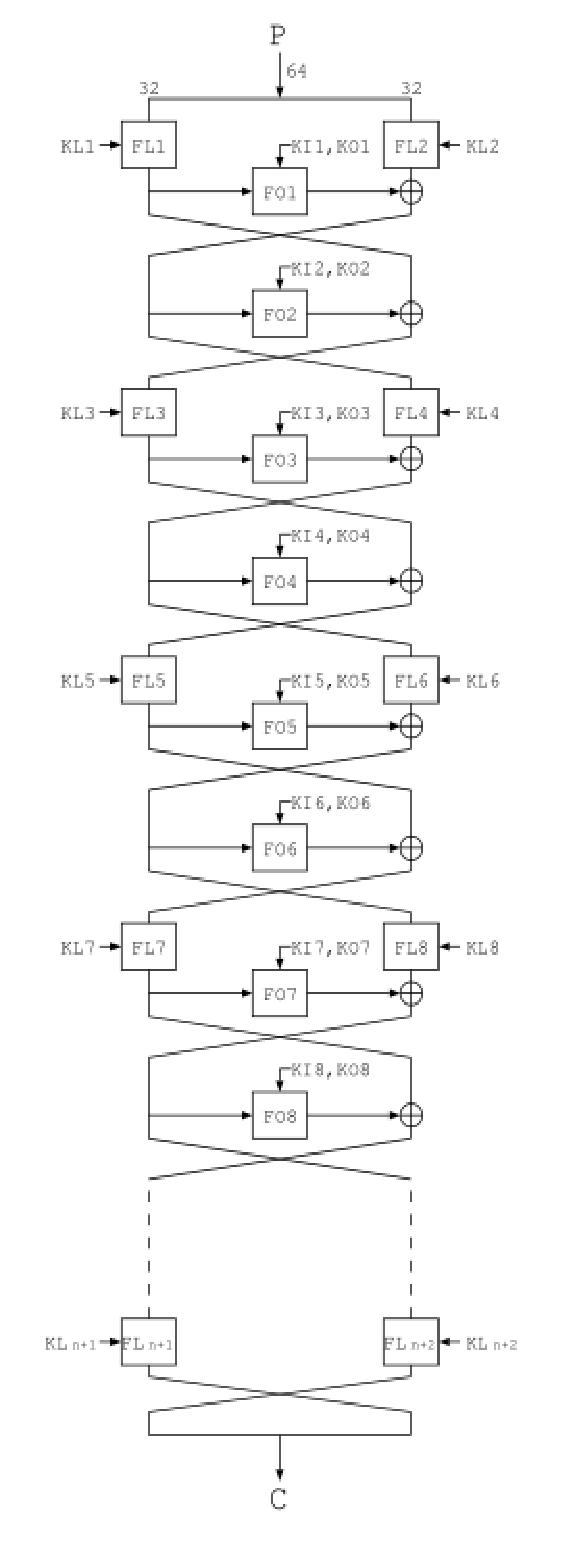
\includegraphics[scale=0.7]{images/misty_feistel}
	\caption{\misty\ cipher structure}
    \label{fig:misty_feistel}
\end{figure}

Key schedule is performed by iterative applying of $FI$ function to each
$16$-bit chunk of the key (figure~\ref{fig:misty_key_schedule}). Hereby $128$
additional subkey bits are generated.  Both the key and the subkey bits are used
during enciphering.

The key injecting function includes conjunction and disjunction operations and
is presented on figure~\ref{fig:misty_fl}.

\begin{figure}[p]
    \begin{subfigure}[b]{0.5\textwidth}
        \centering
        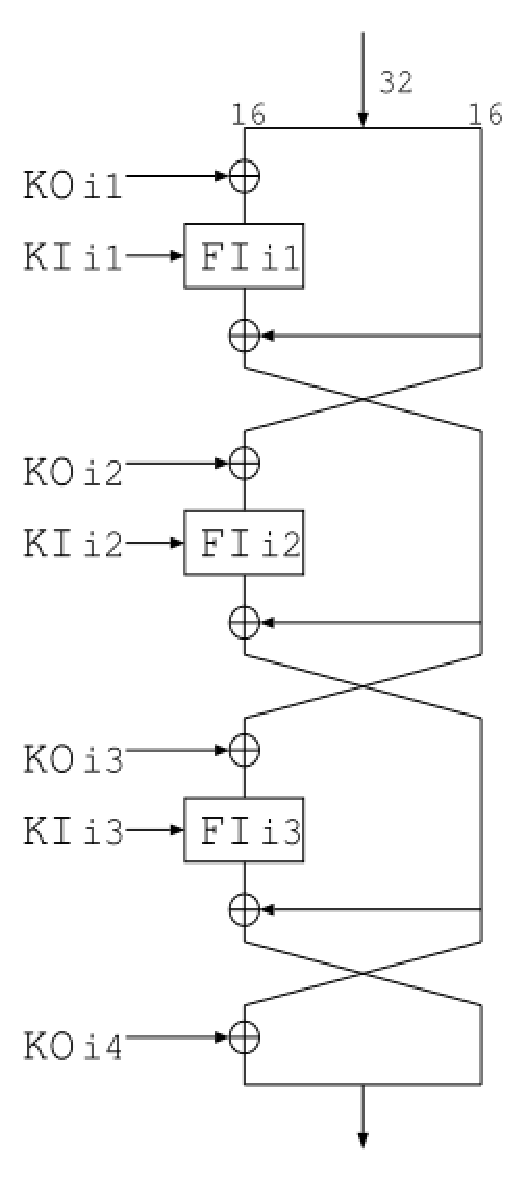
\includegraphics[scale=0.5]{images/misty_fo}
        \caption{$FO$ round function}
        \label{fig:misty_fo}
    \end{subfigure}%
    \begin{subfigure}[b]{0.5\textwidth}
        \centering
        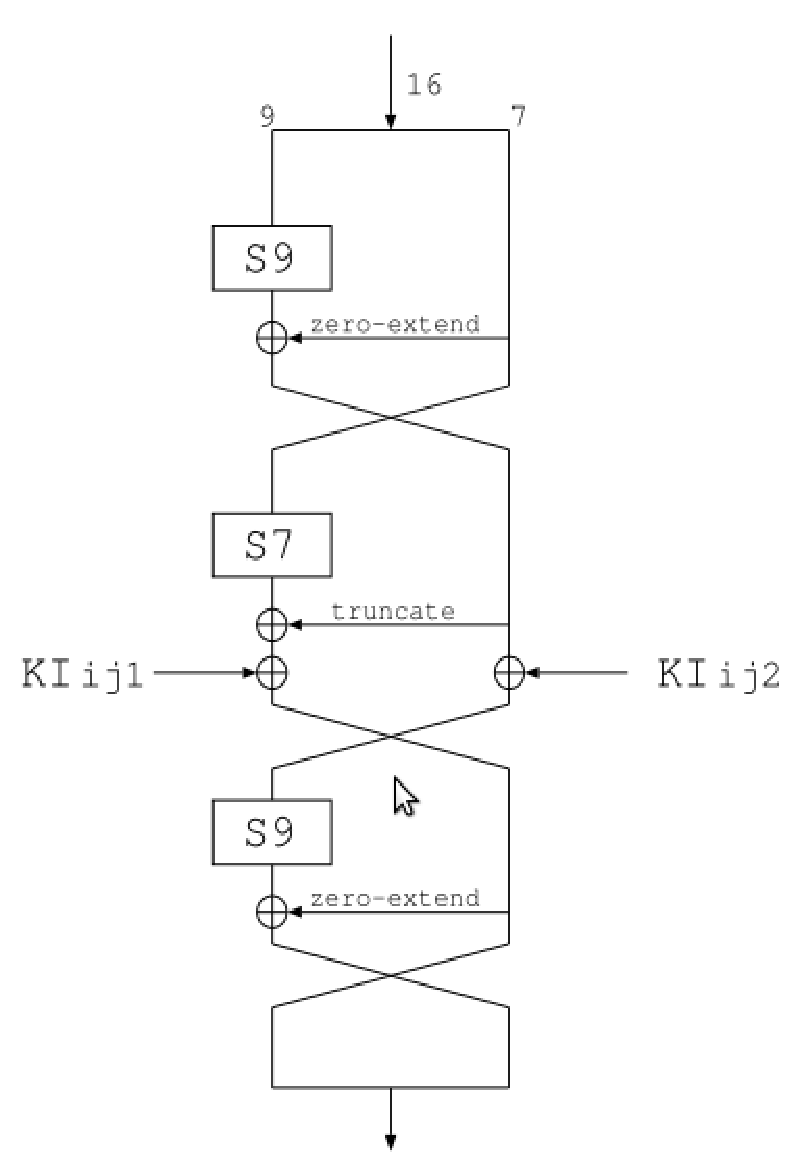
\includegraphics[scale=0.5]{images/misty_fi}
        \caption{$FI$ round function}
        \label{fig:misty_fi}
    \end{subfigure}

    \begin{subfigure}[b]{\textwidth}
        \vspace{1em}
        \centering
        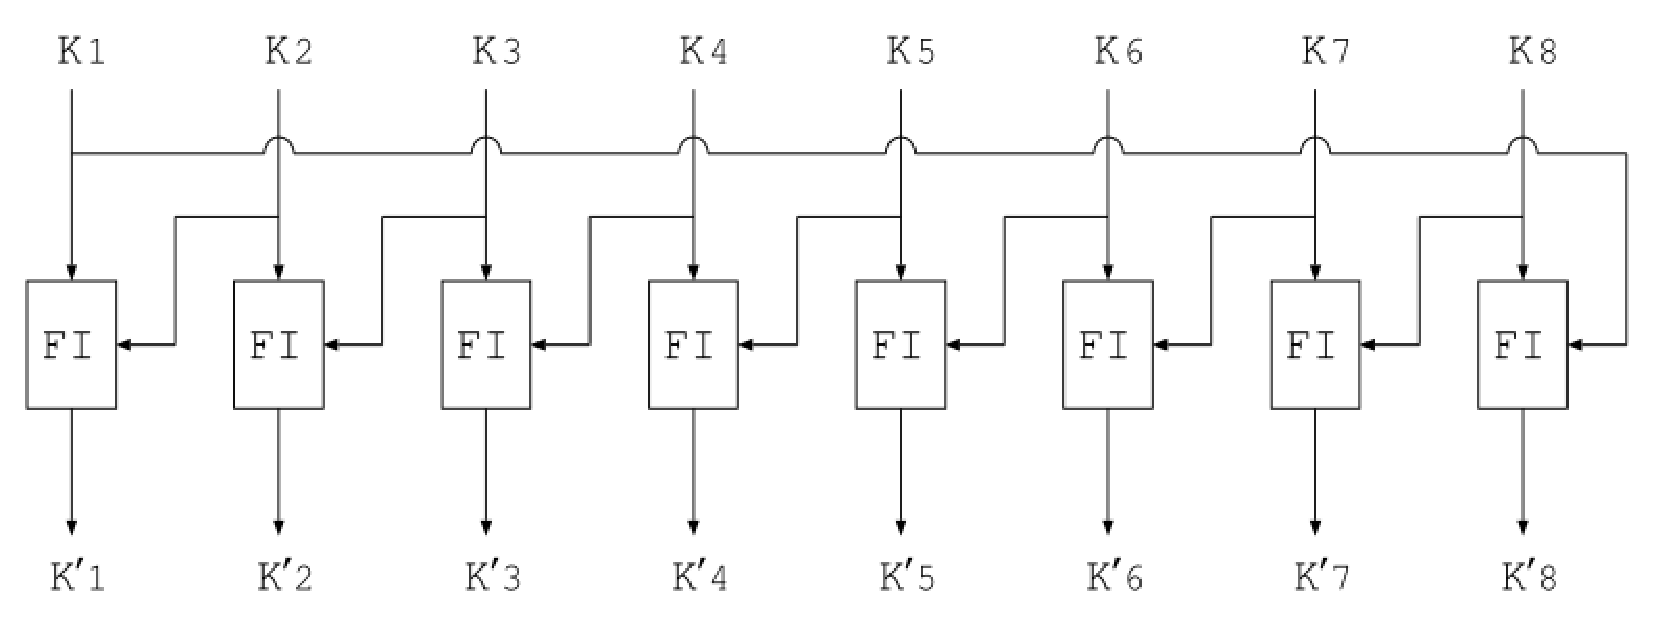
\includegraphics[scale=0.5]{images/misty_key_schedule}
        \caption{Key schedule}
        \label{fig:misty_key_schedule}
    \end{subfigure}
    \caption{\misty\ internal functions}
    \label{fig:misty_round_funcs}
\end{figure}

\begin{figure}[p]
    \centering
    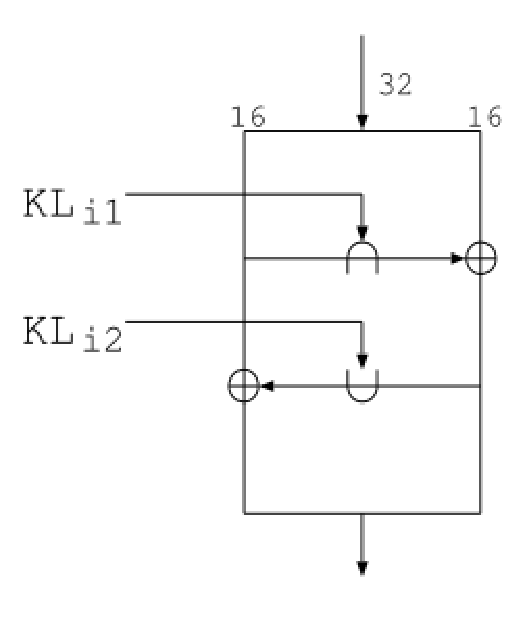
\includegraphics[scale=0.5]{images/misty_fl}
    \caption{Key injection $FL$ function}
    \label{fig:misty_fl}
\end{figure}

S-boxes in \misty\ are constructed algebraically. S-Box $S_7$ has degree $2$ and
$s_9$ is of degree 3. Equations for each S-box are defined in
(\ref{eqn:misty-s7}, \ref{eqn:misty-s9}).

\begin{equation}
    \label{eqn:misty-s7}
    \begin{array}{ll}
        y_0 =& x_0 + x_1 x_3 + x_0 x_3 x_4 + x_1 x_5 + x_0 x_2 x_5 + x_4 x_5 + \\
             & + x_0 x_1 x_6 + x_2 x_6 + x_0 x_5 x_6 + x_3 x_5 x_6 + 1 \\
        y_1 =& x_0 x_2 + x_0 x_4 +x_3 x_4 +x_1 x_5 + x_2 x_4 x_5 +x_6 + \\
             & + x_0 x_6 +x_3 x_6 +x_2 x_3 x_6 + x_1 x_4 x_6 + x_0 x_5 x_6 +1 \\
        y_2 =& x_1 x_2 + x_0 x_2 x_3 + x_4 + x_1 x_4 + x_0 x_1 x_4 + x_0 x_5 + x_0 x_4 x_5 + \\
             & + x_3 x_4 x_5 + x_1 x_6 + x_3 x_6 + x_0 x_3 x_6 + x_4 x_6 + x_2 x_4 x_6 \\
        y_3 =& x_0 + x_1 + x_0 x_1 x_2 + x_0 x_3 + x_2 x_4 + x_1 x_4 x_5 + \\
             & + x_2 x_6 + x_1 x_3 x_6 + x_0 x_4 x_6 + x_5 x_6 + 1 \\
        y_4 =& x_2 x_3 + x_0 x_4 + x_1 x_3 x_4 + x_5 + x_2 x_5 + x_1 x_2 x_5 + \\
             & + x_0 x_3 x_5 + x_1 x_6 + x_1 x_5 x_6 + x_4 x_5 x_6 + 1 \\
        y_5 =& x_0 + x_1 + x_2 + x_0 x_1 x_2 + x_0 x_3 + x_1 x_2 x_3 + x_1 x_4 + \\
             & + x_0 x_2 x_4 + x_0 x_5 + x_0 x_1 x_5 + x_3 x_5 + x_0 x_6 + x_2 x_5 x_6 \\
        y_6 =& x_0 x_1 + x_3 + x_0 x_3 + x_2 x_3 x_4 + x_0 x_5 + x_2 x_5 + \\
             & + x_3 x_5 + x_1 x_3 x_5 + x_1 x_6 + x_1 x_2 x_6 + x_0 x_3 x_6 + x_4 x_6 + x_2 x_5 x_6 \\
    \end{array}
\end{equation}

\begin{equation}
    \label{eqn:misty-s9}
    \begin{array}{ll}
        y_0 =& x_0 x_4 + x_0 x_5 + x_1 x_5 + x_1 x_6 + x_2 x_6 + x_2 x_7 + \\
             & + x_3 x_7 + x_3 x_8 + x_4 x_8 + 1 \\
        y_1 =& x_0 x_2 + x_3 + x_1 x_3 + x_2 x_3 + x_3 x_4 + x_4 x_5 + x_0 x_6 + \\
             & + x_2 x_6 + x_7 + x_0 x_8 + x_3 x_8 + x_5 x_8 +1 \\
        y_2 =& x_0 x_1 + x_1 x_3 + x_4 + x_0 x_4 + x_2 x_4 + x_3 x_4 + x_4 x_5 + \\
             & + x_0 x_6 + x_5 x_6 + x_1 x_7 + x_3 x_7 + x_8 \\
        y_3 =& x_0 + x_1 x_2 + x_2 x_4 + x_5 + x_1 x_5 + x_3 x_5 + x_4 x_5 + \\
             & + x_5 x_6 + x_1 x_7 + x_6 x_7 + x_2 x_8 + x_4 x_8 \\
        y_4 =& x_1 + x_0 x_3 + x_2 x_3 + x_0 x_5 + x_3 x_5 + x_6 + x_2 x_6 + \\
             & + x_4 x_6 + x_5 x_6 + x_6 x_7 + x_2 x_8 + x_7 x_8 \\
        y_5 =& x_2 + x_0 x_3 + x_1 x_4 + x_3 x_4 + x_1 x_6 + x_4 x_6 + x_7 + \\
             & + x_3 x_7 + x_5 x_7 + x_6 x_7 + x_0 x_8 + x_7 x_8 \\
        y_6 =& x_0 x_1 + x_3 + x_1 x_4 + x_2 x_5 + x_4 x_5 + x_2 x_7 + x_5 x_7 + \\
             & + x_8 + x_0 x_8 + x_4 x_8 + x_6 x_8 + x_7 x_8 +1 \\
        y_7 =& x_1 + x_0 x_1 + x_1 x_2 + x_2 x_3 + x_0 x_4 + x_5 + x_1 x_6 + \\
             & + x_3 x_6 + x_0 x_7 + x_4 x_7 + x_6 x_7 + x_1 x_8 +1 \\
        y_8 =& x_0 + x_0 x_1 + x_1 x_2 + x_4 + x_0 x_5 + x_2 x_5 + x_3 x_6 + \\
             & + x_5 x_6 + x_0 x_7 + x_0 x_8 + x_3 x_8 + x_6 x_8 +1 \\
    \end{array}
\end{equation}


\section{Construction of equations system for \misty}

\misty is a $64$-bit Feistel network similar to \gost and doesn't use any
additional operations that are not described in~\ref{sec:equations}, there for
construction of equations is performed similarly.

There are few differences however. Even though the transformations used in
\misty\ are resembling those of \gost\, its structure is much more complicated
due to nested Feistel networks. Initially equations for each function are
constructed and tested for correctness so that definition of each Feistel
network is self-contained. Afterwards those equations are chained into single
system as usually.

Since \misty uses key scheduling, equations for this transformation also must be
explicitly defined.

Nested structure of \misty\ results in big number of variables so they must be
named carefully to avoid confusion. The following format was used for \misty\
variables: \verb+R<n>_<func>_<op>_<bit>+, where \verb+n+ denotes number of
current round, \verb+func+ stands for function to which variable belongs,
\verb+op+ is some operation inside the function, \verb+bit+ is the number of bit
in a block. For example variable \verb+verb+n+ denotes number of
current round, \verb+func+ stands for function to which variable belongs,
\verb+op+ is some operation inside the function, \verb+bit+ is the number of bit
in a block. For example variable \verb+R5_FO_KO2_15+ stands for round $5$,
function $FO$, operation of injecting subkey $KO_{i2}$, precisely bit $15$ of
the subkey.

Using the described method the full-scale system of equations for \misty\
has been constructed and shown to have $3488$ equations in $3680$ variables.
Because of nested structure too many
variables are introduced and the system becomes underdefined and therefore
unsolvable. To overcome such problem it is possible to apply Gr\"obner basis
(described in~\ref{sec:groebner}) to some transformation for obtaining more
equations and possibly eliminating some of the variables. It has been decided to
post-process equations for S-box $S_7$ by computing the corresponding
Gr\"obner basis. The resulting system has $8448$ equations in $3680$ variables,
so usage of Gr\"obner basis introduced another $5000$ equations.


\subsection{Key recovery for 2 rounds of \misty}
\label{sec:misty-key-rec}

For the attack $4$ systems of equations for distinct
\mbox{plaintext/ciphertext} pairs have been combined in order for
the number of known values to reach the unicity distance.

With the use of \verb+CryptoMiniSat+ solver on a low-end computer an equations
system for two \misty\ rounds have successfully been solved and the used subkeys
recovered. For the system of $4$ rounds equivalent keys can be obtained for a
given \mbox{plaintext/ciphertext} pair.

Further combinations of Gr\"obner basis technique with SAT-solvers and
usage of powerful computers may refine the efficiency of the attack and provide
more capabilities for analyzing properties of the cryptoalgorithm.


\section{Summary}

The chapter provides description of constructing systems of non-linear equations
for cryptoalgorithms \gost\ and \misty\ that are based on Feistel network and
some approaches for solving the obtained equations set.

Gr\"obner basis method generally is not efficient enough for solving full-scale
equations system but is useful for obtaining exhaustive list of linearly
independent equations for given transformation. It is especially beneficial for
S-box equations.

With advance of SAT-solver algorithms they become efficient enough for solving
large equations sets and with the help of powerful computers it might be
possible to solve system of equations for some full-scale cipher. The downside
of such algorithms is their nondetermination and therefore no guarantee of
average run time for given instance. This exaggerates complexity evaluation of
solving given equations set and one can only predict the overall complexity of
the problem based on preliminary characteristics of equations set (degree,
number of equations and variables, etc.) and estimate the possibility of its
solving but cannot bind these factors to some certain time complexity of the
attack.

Using the proposed methods for defining symmetric ciphers with equations set,
polynomial system for \misty\ has $8448$ equations in $3680$ variables
and the system for \gost\ has $10432$ equations in $4416$ variables.
For comparison, the polynomial system for the PRESENT cipher that is
designed for lightweight cryptography purposes contains $11067$ quadratic
equations in $4216$ variables~\cite{ches:present:2007}. Even though PRESENT has
very simple structure, its equations system is larger. But also PRESENT has much
smaller key space and requires more space for hardware implementation. It is
claimed that AES cipher can be described with an algebraic system of $8000$
quadratic equations in $1600$ unknowns~\cite{cid2006algebraic} which is
signivicantly smaller than the \gost\ or \misty\ equations system. An equations
set for symmetric block cipher Camellia contains $6224$ equations in $3584$
variables~\cite{Biryukov03blockciphers}.

